%%%%%%%%%%%%%%%%%%%%%%%%%%%%%%%%%%%%%%%%%%%%%%%%%%
% Basic setup. Most papers should leave these options alone.
\documentclass[fleqn,usenatbib]{mnras}

% MNRAS is set in Times font. If you don't have this installed (most LaTeX
% installations will be fine) or prefer the old Computer Modern fonts, comment
% out the following line
%\usepackage{newtxtext,newtxmath}
% Depending on your LaTeX fonts installation, you might get better results with one of these:
%\usepackage{mathptmx}
%\usepackage{txfonts}
% 
% Use vector fonts, so it zooms properly in on-screen viewing software
% Don't change these lines unless you know what you are doing
% \usepackage[T1]{fontenc}

% Allow "Thomas van Noord" and "Simon de Laguarde" and alike to be sorted by "N" and "L" etc. in the bibliography.
% Write the name in the bibliography as "\VAN{Noord}{Van}{van} Noord, Thomas"
\DeclareRobustCommand{\VAN}[3]{#2}
\let\VANthebibliography\thebibliography
\def\thebibliography{\DeclareRobustCommand{\VAN}[3]{##3}\VANthebibliography}


%%%%% AUTHORS - PLACE YOUR OWN PACKAGES HERE %%%%%

% Only include extra packages if you really need them. Common packages are:
\usepackage{graphicx}	% Including figure files
\usepackage{amsmath}	% Advanced maths commands
\usepackage{amssymb}	% Extra maths symbols

%%%%%%%%%%%%%%%%%%%%%%%%%%%%%%%%%%%%%%%%%%%%%%%%%%

%%%%% AUTHORS - PLACE YOUR OWN COMMANDS HERE %%%%%

% Please keep new commands to a minimum, and use \newcommand not \def to avoid
% overwriting existing commands. Example:
%\newcommand{\pcm}{\,cm$^{-2}$}	% per cm-squared


\newcommand{\Rcon}{R_{T=10^5\,{\rm K}}}
\newcommand{\tcon}{t_{T=10^5\,{\rm K}}}
\newcommand{\Mdot}{\dot{M}}
\newcommand{\Rcirc}{R_{\rm circ}} %need better name as R_cool means something else
\newcommand{\Rvir}{R_{\rm vir}}
\newcommand{\nH}{n_{\rm H}}
\newcommand{\Tvir}{T_{\rm vir}}
\newcommand{\msun}{{\rm M}_\odot}
\newcommand{\vvir}{v_{\rm vir}}

%%%%%%%%%%%%%%%%%%%%%%%%%%%%%%%%%%%%%%%%%%%%%%%%%%

%%%%%%%%%%%%%%%%%%% TITLE PAGE %%%%%%%%%%%%%%%%%%%

% Title of the paper, and the short title which is used in the headers.
% Keep the title short and informative.
\title[Quiet Accretion onto $L^*$ Galaxies]{The Quiet Fueling of MW-Like Disks}

% James suggestions: Go super big. This is a grand challenge, we're trying to tackle it.
% Potential title: Circularized cooling flows and the formation of thin disk galaxies
% Frame as grand challenge in galaxy formation.
% Only able to form thin disks recently, but why?
% Well, now we know.
% Open mysteries about thin disk formation in circumstances where galaxies don't have this accretion mode.
% Suggests the nature of the CGM is fundamental to galaxy morphology.

% Big framing because we don't want this to be thought of as a detail.

% The list of authors, and the short list which is used in the headers.
% If you need two or more lines of authors, add an extra line using \newauthor
\author[Hafen, Stern, Bullock et al.]{
Zachary Hafen,$^{1}$\thanks{E-mail: zhafen@uci.edu}
Jonathan Stern,
James Bullock,
\ldots
\\
% List of institutions
$^1$,
\ldots
}

% These dates will be filled out by the publisher
\date{Accepted XXX. Received YYY; in original form ZZZ}

% Enter the current year, for the copyright statements etc.
\pubyear{2020}

% Don't change these lines

\begin{document}
\label{firstpage}
\pagerange{\pageref{firstpage}--\pageref{lastpage}}
\maketitle

% Abstract of the paper
\begin{abstract}
We study how gas accretes onto $\sim L^\star$ star-forming galaxies at redshift $z\sim0$ using FIRE cosmological simulations.
We find three primary characteristics:
(i) hot virial temperature gas dominates ($\gtrsim80\%$) the inflowing gas mass on halo scales ($\gtrsim 20$ kpc);
(ii) accreting gas cools at the galaxy-halo interface, with the peak of the cooling occuring just outside the galaxy;
(iii) cooling and circularization occur simultaneously; accretion transitions from a hot quasi-spherical configuration to a cool disc-like configuration over the course of $\lesssim 200$ Myr.
This accretion mode, which we refer to as \textit{quiet accretion}, occurs when volume-filling, stable gas reaches the radius at which it is rotationally-supported.
The rotational support increases density and prevents compressive heating, inducing rapid cooling.
Prior to cooling the volume-filling gas equilibriates to a coherent rotation.
Subsequently when the gas cools it forms a disk that is on-average co-rotating with the galaxy.
Quiet accretion is expected to be more conducive to disk formation than other modes of accretion, and is a general outcome of a radiatively cooling hot volume-filling CGM phase.
% We evaluate the relative importance of three different modes of accretion: 
% gas that never heats to the virial temperature (``cold accretion''), 
% cool clouds which condense out of the hot halo, lose buoyancy and accrete  (``condensation''), 
% and inflowing hot gas which remains hot down to the galaxy scale (``cooling flow'').
% We demonstrate that across our sample of MW-mass halos most accretion occurs via a cooling flow.
% % We demonstrate that across our sample of $xx$ MW-mass halos most accretion occurs via a cooling flow, accounting for $yy-zz\%$ of all accreted gas. % Put this back in when we know the numbers
% Gas accreted in this mode is hot and quasi-spherical down to when it becomes rotationally-supported at $\lesssim 0.1$ of the halo virial radius.
% After becoming rotationally-supported it simultaneously cools and circularizes, thus joining the outskirts of the galactic disc. 
% % Only a small fraction ($zz$\%) of this hot flow experienced condensation and reheating prior to accretion. 
% % The remaining $vv-ww\%$ of accreted gas originates in cool clouds which condensed out of the halo. Cold accretion does not occur in appreciable quantities at $z\sim0$ in our simulations.
% \textbf{
% Include: Compare Mdotcool with the accretion rate and SFR to further strengthen the relation, maybe through Figure 1 in an energetic sense.
% }
\end{abstract}

% Select between one and six entries from the list of approved keywords.
% Don't make up new ones.
\begin{keywords}
galaxies: disc -- galaxies: evolution -- galaxies: halos -- cosmology: theory
\end{keywords}

%%%%%%%%%%%%%%%%%%%%%%%%%%%%%%%%%%%%%%%%%%%%%%%%%%

%%%%%%%%%%%%%%%%% BODY OF PAPER %%%%%%%%%%%%%%%%%%

% INTUITIVE OVERVIEW
\begin{figure*}
    \centering
    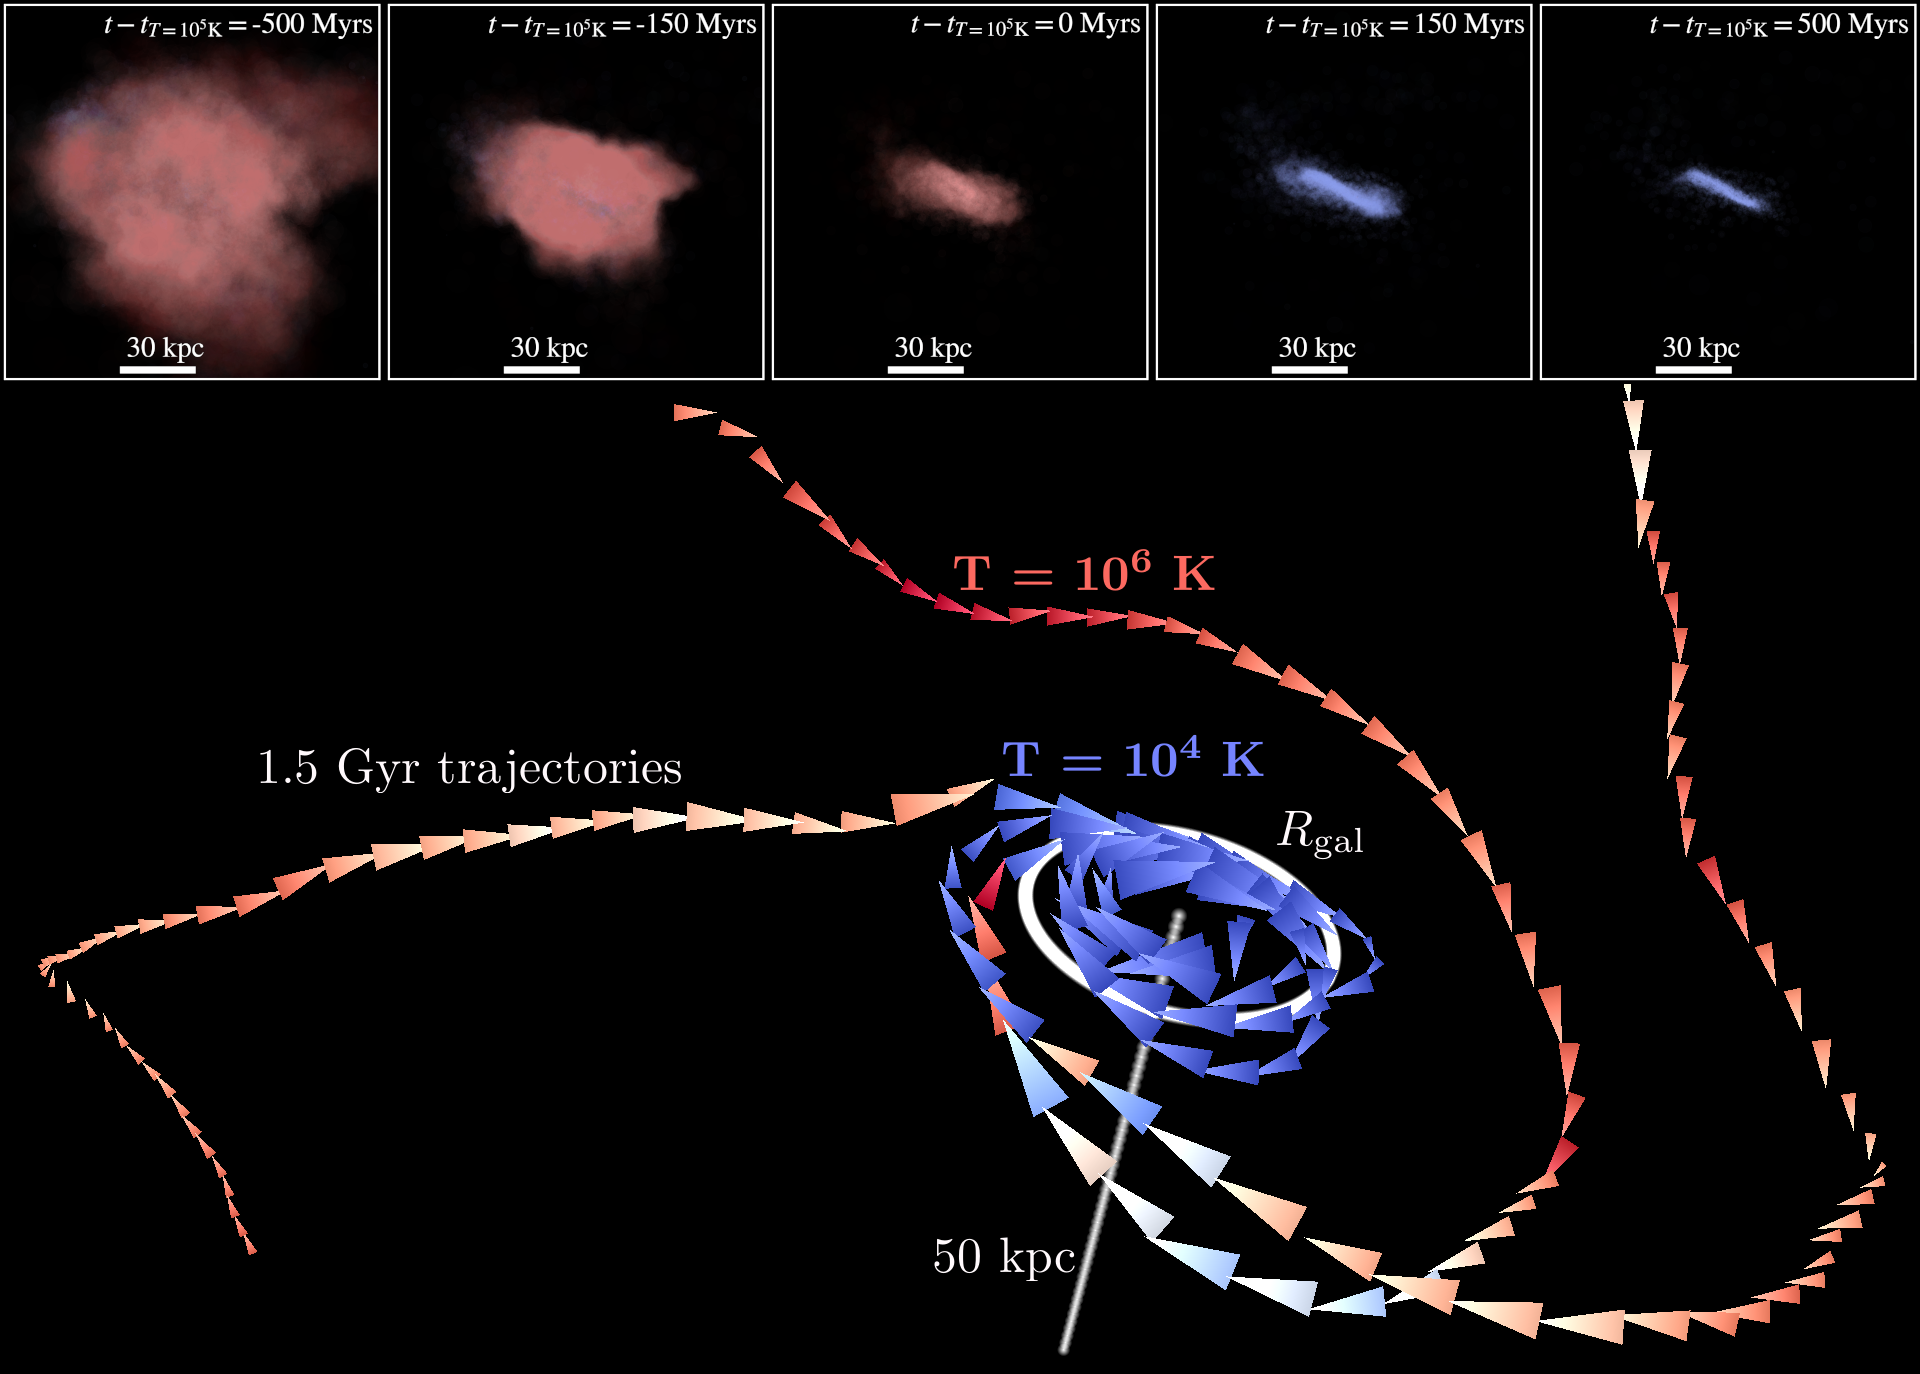
\includegraphics[width=\textwidth]{figures/illustrative_tracks/illustrative_tracks.png}
    \caption{
Example trajectories showing how gas accretes onto Milky-Way mass disc galaxies at $z\approx0$ in FIRE.
Trajectories are representative of gas that is outside a Milky-Way-like galaxy one Gyr prior to $z=0$, and inside the galaxy at $z=0$.
% We show the trajectories for 1 Gyr prior to the final time gas cools below $T=10^5$ K prior to accreting onto the galaxy, and 0.5 Gyr after cooling.
The trajectories are characteristic of \textit{quiet accretion}:
Accreted gas is hot and voluminous until it cools at the galaxy-halo interface, at which time it also forms a rotating disc structure.
    }
    \label{f: overview}
\end{figure*}


% HOT IN HALO
\begin{figure*}
    \centering
    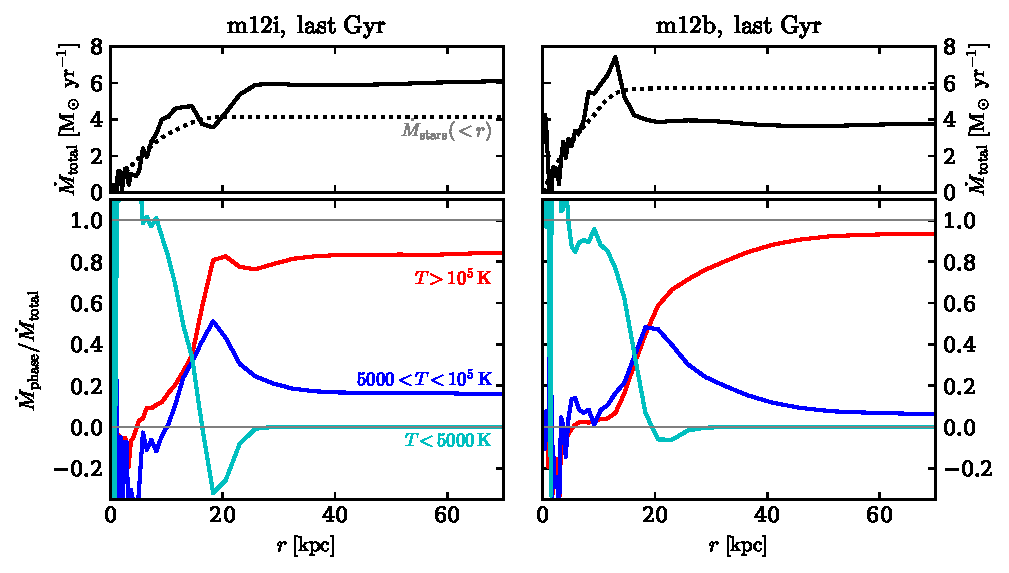
\includegraphics{figures/Mdot_normalized.pdf}
    \caption{
    Average mass inflow rate over the course of one Gyr prior to $z=0$ in two $\sim L^\star$ FIRE halos.
    Black lines in the top panels show the total mass inflow rate while colored lines in the bottom panels show the division into the hot, cool and cold phases.
    The dotted line in the top panel shows the rate of gas conversion into stars within a given radius.
    The hot phase dominates the mass inflow in these halos, down to the galaxy scale of $\approx15$ kpc.
    \textbf{Verify conversion SFR to Mdot\_stars, add SFR of satellites}
    \textbf{Try adding labels relative to $T_{\rm vir}$ (Drummond's suggestion).}
    \textbf{Consider removing top panels, as scientists who are very aware of SFR discrepancies may become fixated.}
    \textbf{Use consistent r notation (caps vs not, units in brackets vs parenthesis.).}
    \textbf{Add top x-axis with radius in units of $\Rvir$}.
    }
    \label{f: Mdot}
\end{figure*}

% COOLS AT DISK INTERFACE
\begin{figure*}
    \centering
    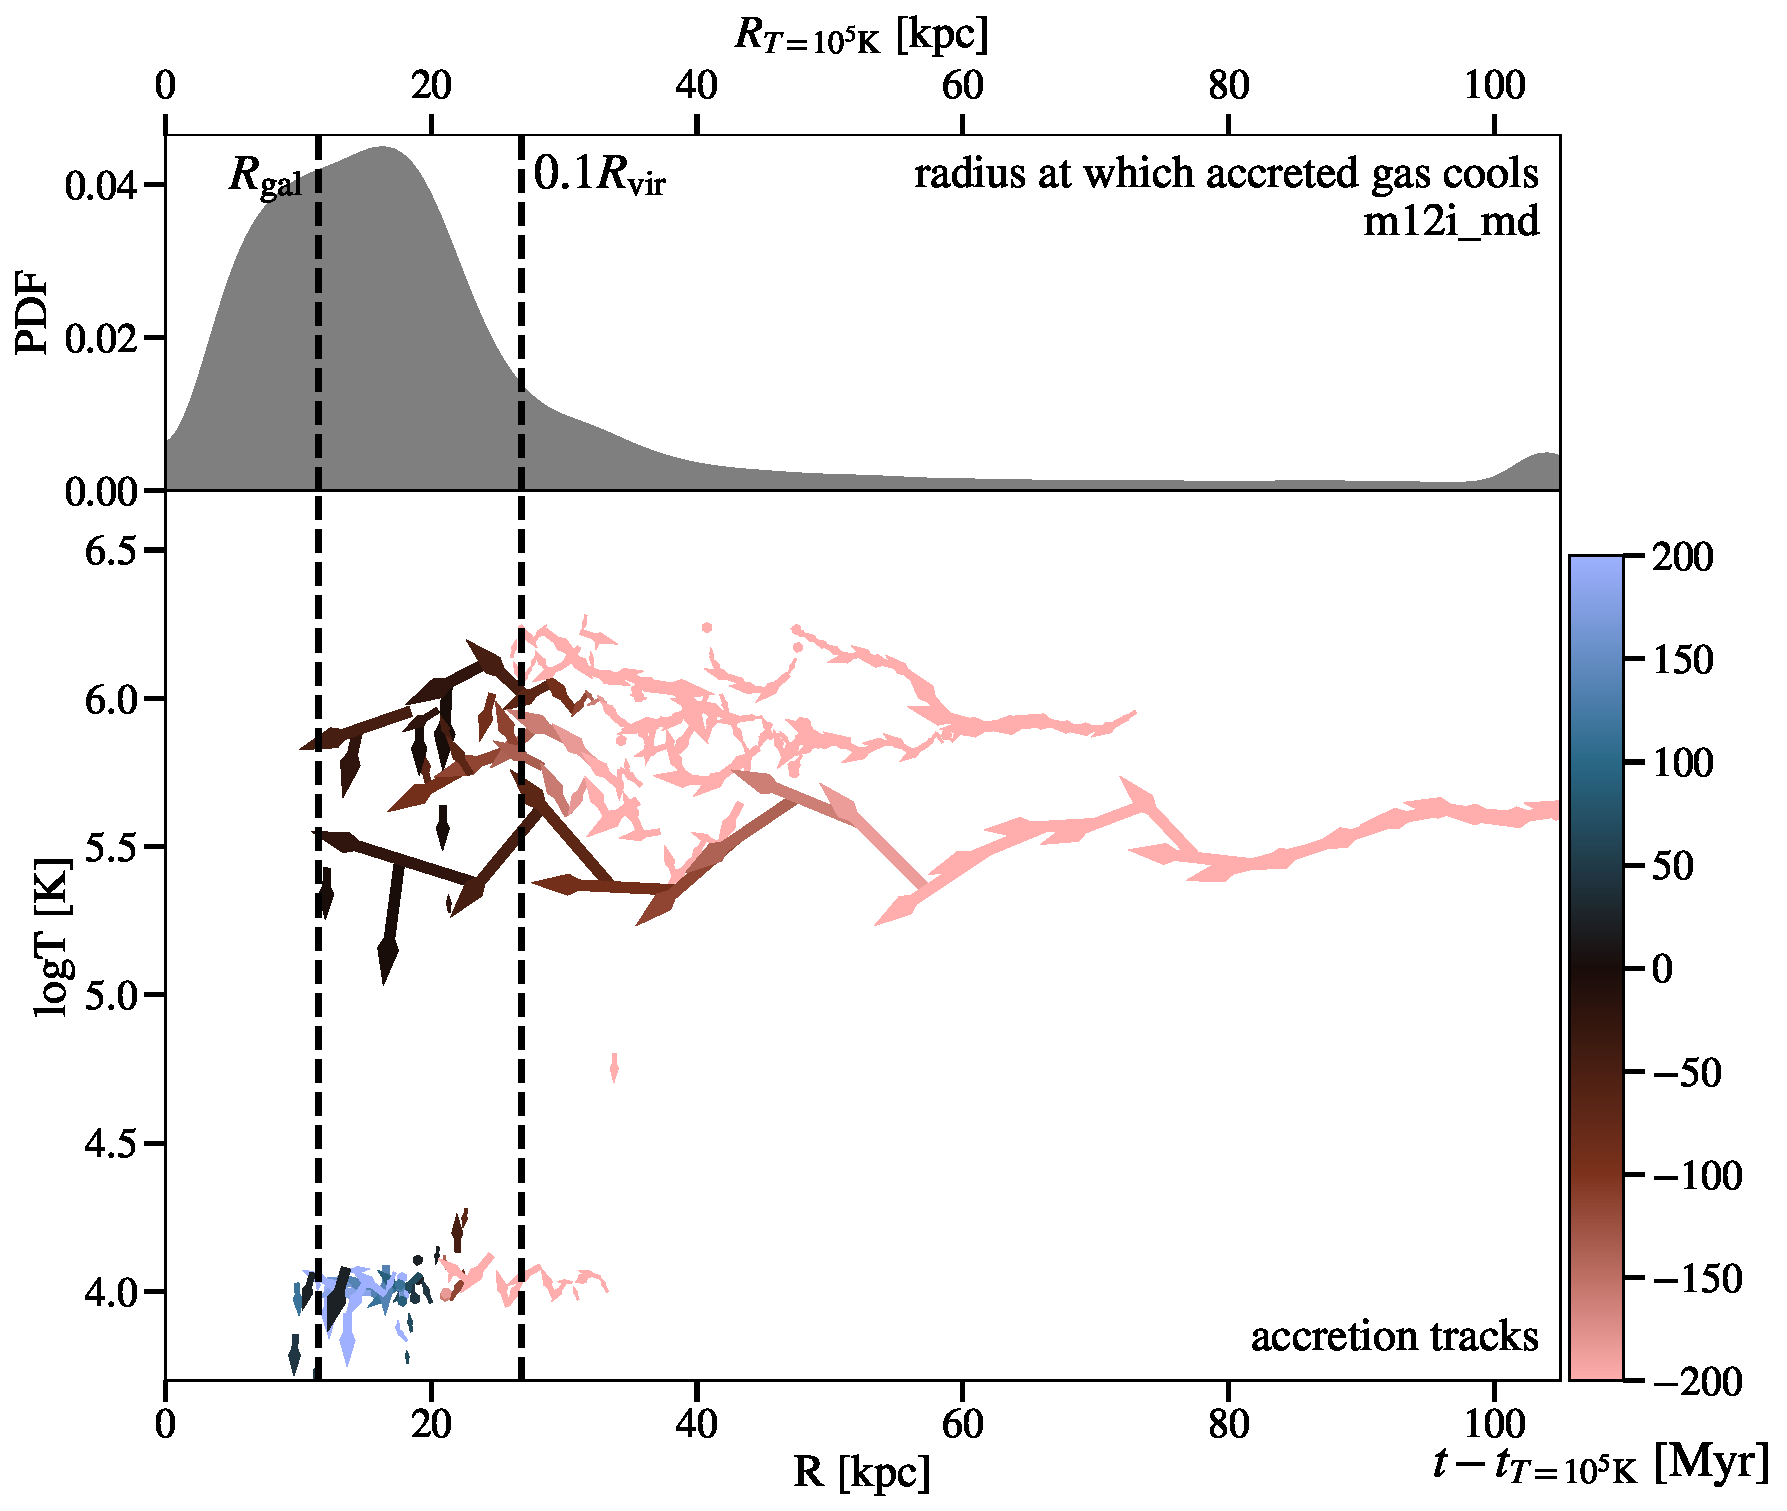
\includegraphics[width=\columnwidth]{figures/tracks/tracks_m12i_md.pdf}
    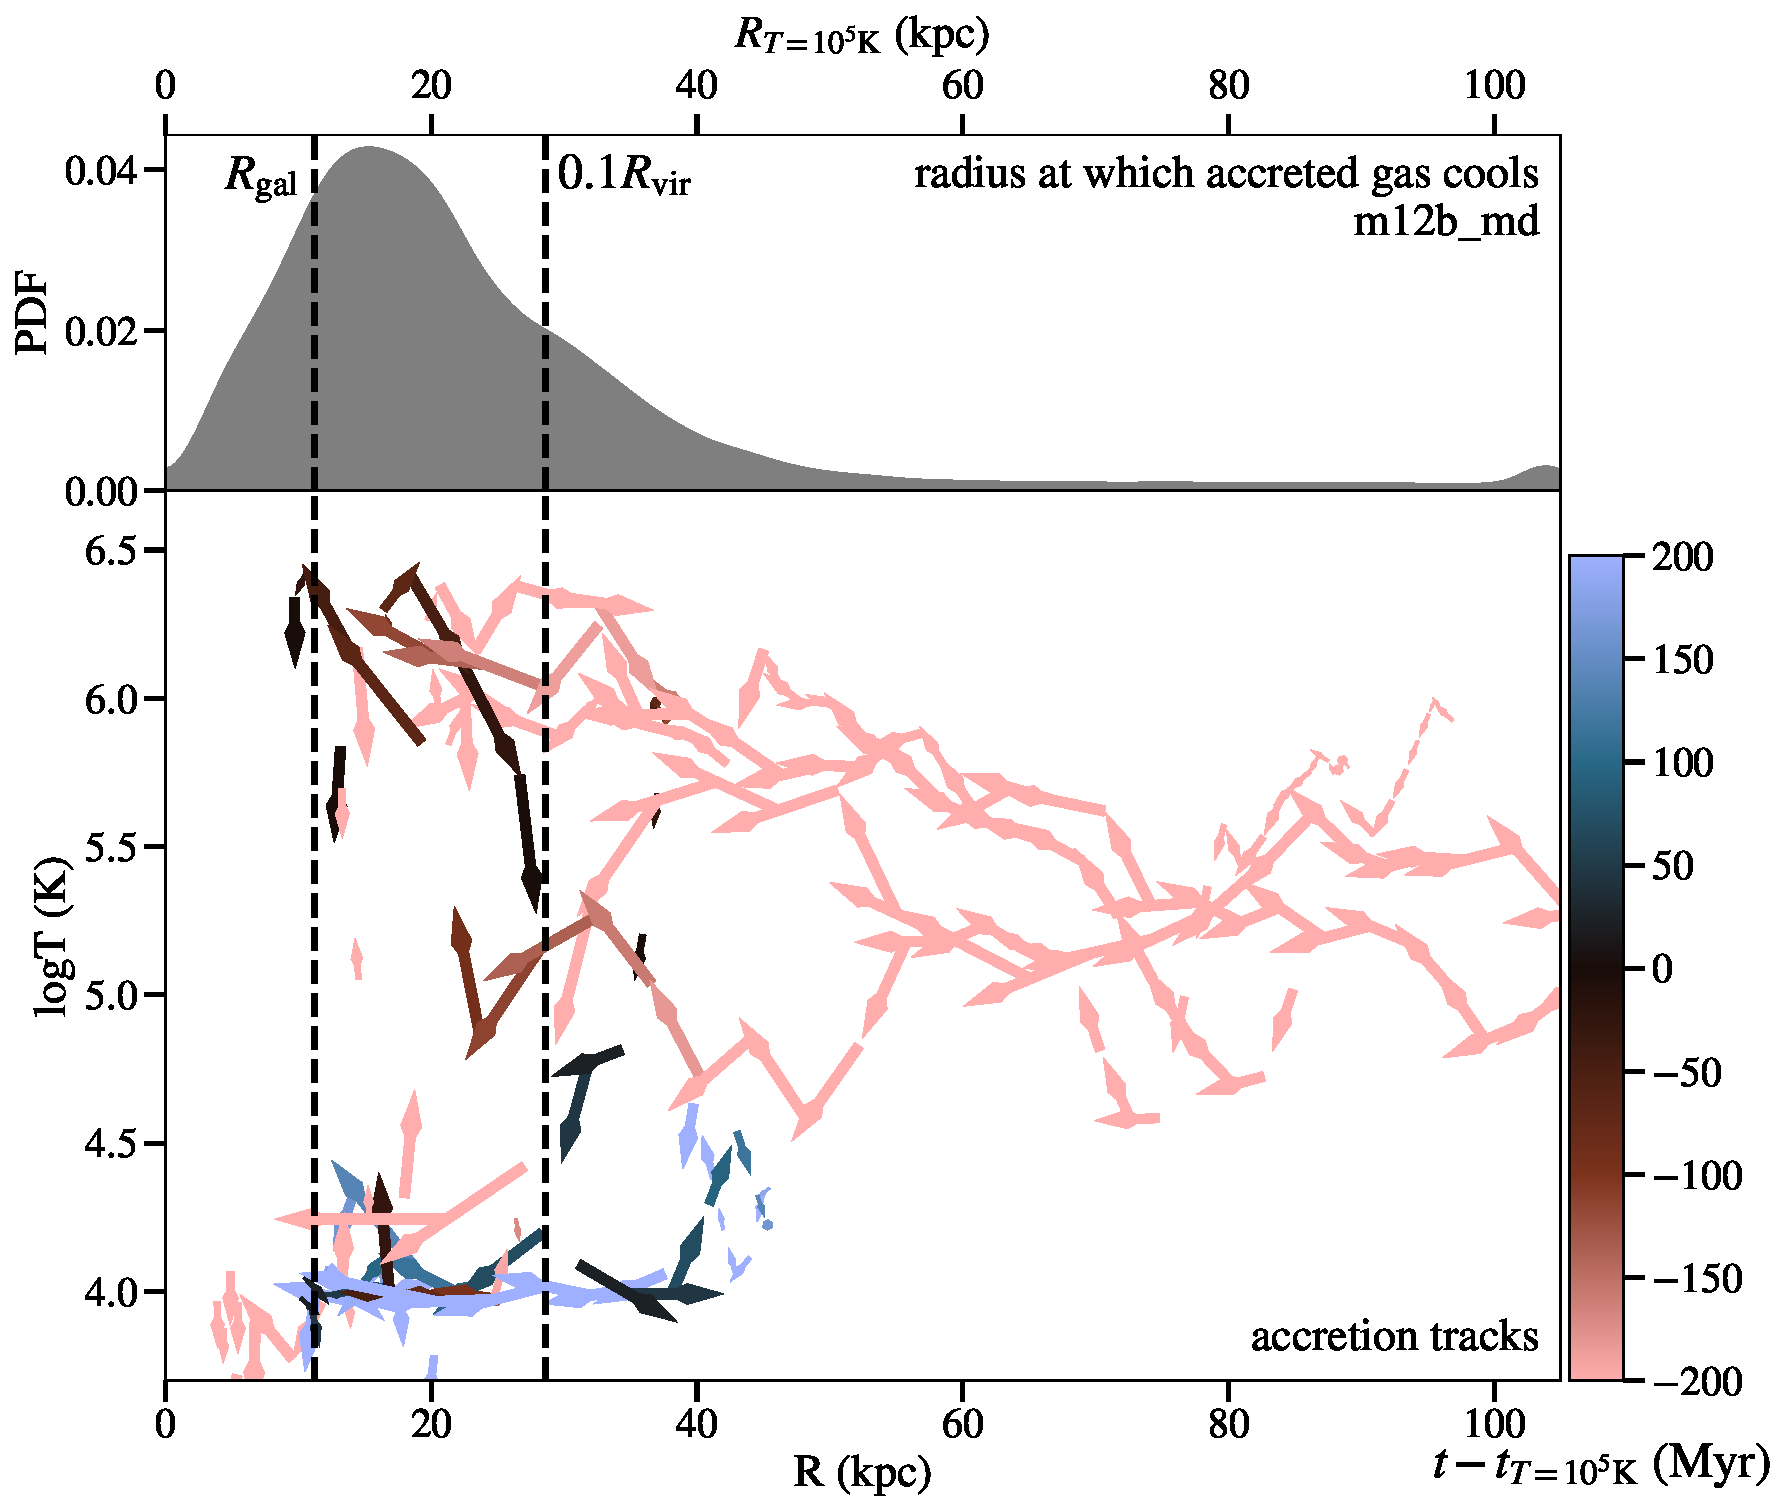
\includegraphics[width=\columnwidth]{figures/tracks/tracks_m12b_md.pdf}
    \caption{
    Radial and temperature trends for gas accreting onto two $L^\star$ FIRE halos at $z\approx0$.
    \textbf{Top panels:} Distribution of $\Rcon$, the radius at which gas particles last cooled below $T=10^5$ K prior to accreting.
    \textbf{Bottom:} Temperature vs radius tracks for five randomly-selected particles per halo, with color indicating time relative to the time at which gas cools.
    At $r \gtrsim 0.1 R_{\rm vir}$ accreted gas either remains hot or cools only temporarily.
    \textbf{
    Consider plotting an edge-on image of the system to-scale above the histogram.
    }
    }
    \label{f: T vs R}
\end{figure*}

% ORIENTS AS IT COOLS
\begin{figure*}
    \centering
    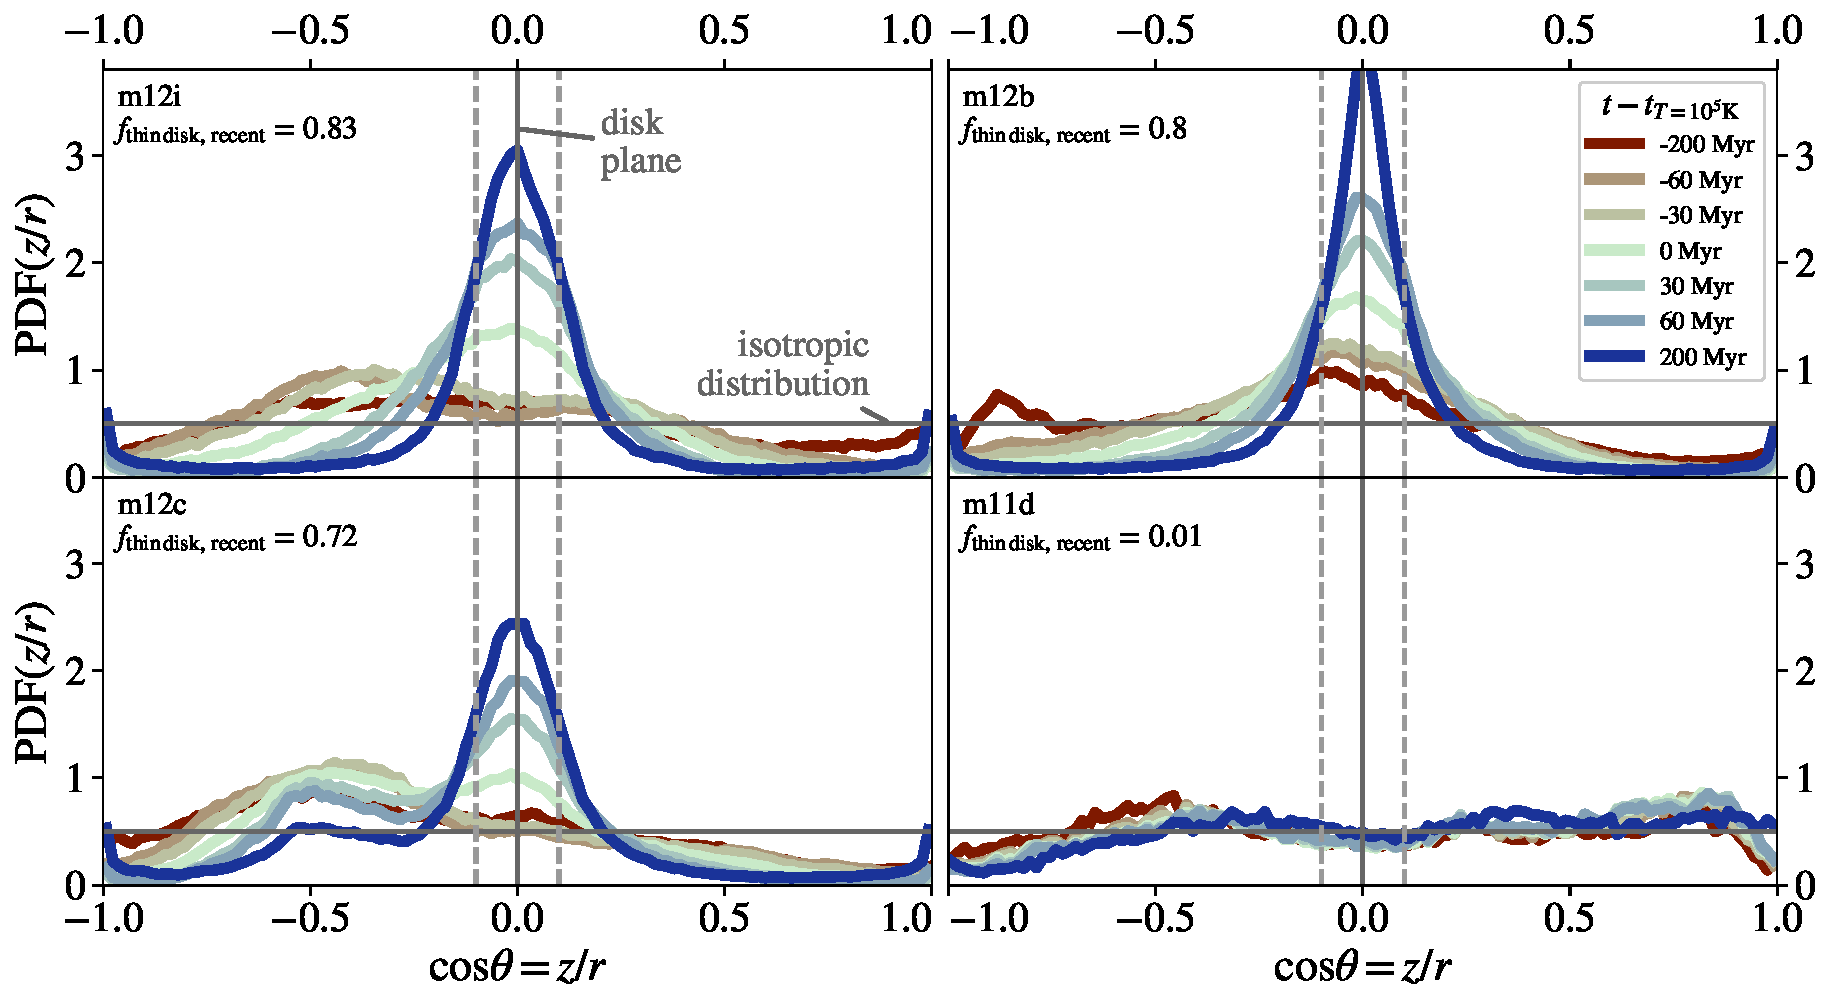
\includegraphics[width=\textwidth]{figures/theta_vs_t.pdf}
    \caption{
    Vertical distribution of accreting gas over 150 Myr before/after cooling for three MW-mass FIRE galaxies and one LMC-mass central galaxy (\texttt{m11d\_md}).
    Angle is relative to the stellar disk, with $z/R = \cos\theta=0$ for gas along the disk plane.
    For $\sim L^*$ galaxies accreting gas is quasi-spherical prior to cooling.
    After cooling the gas has a disc-like configuration, indicating that cooling and circularization occur simultaneously. 
    In contrast, in the lower-mass halo the gas is quasi-spherical both prior to and after cooling, indicating that cooling is not associated with circularization.
    }
    \label{f: theta vs t}
\end{figure*}

% MECHANICS OF QUIET ACCRETION
\begin{figure*}
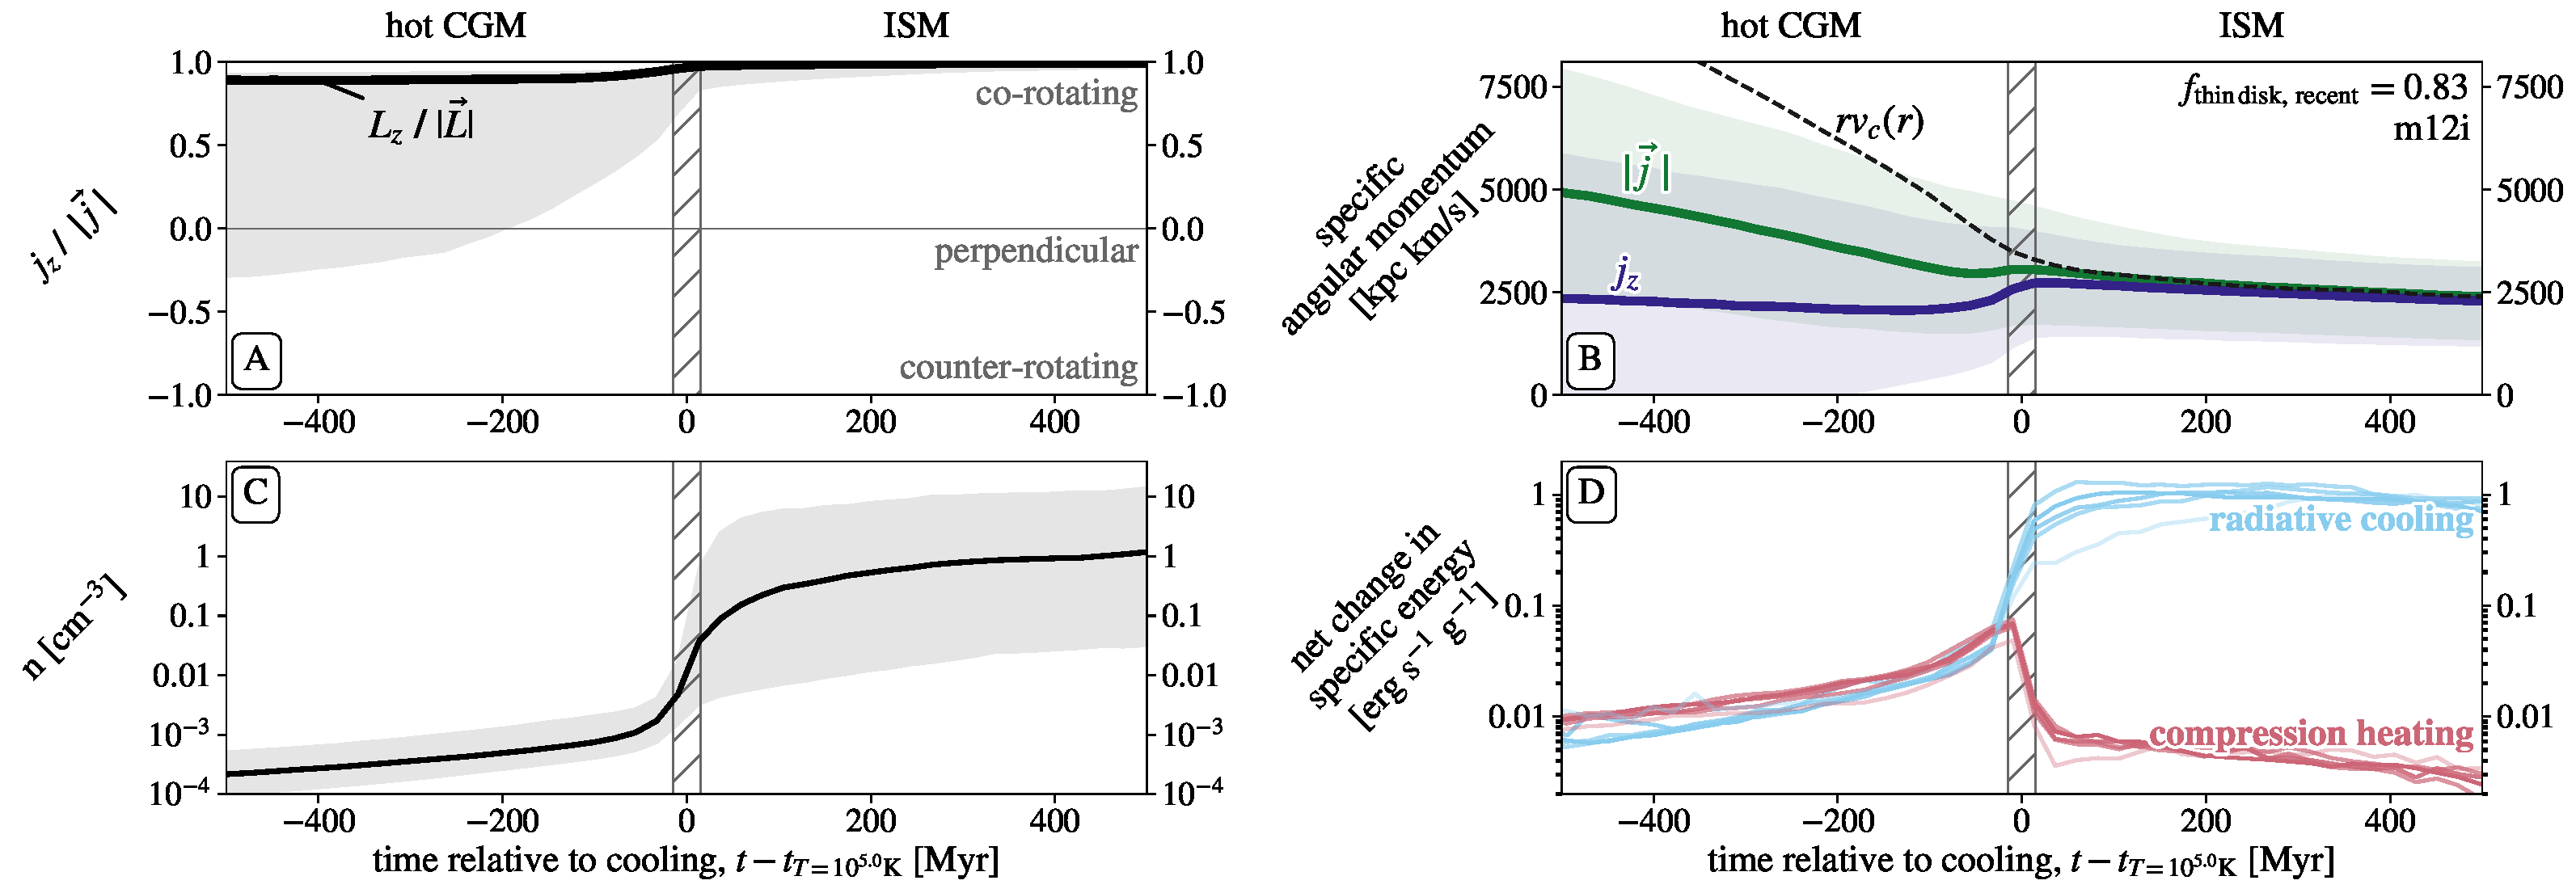
\includegraphics[height=0.75\textheight]{figures/before_and_after/before_and_after_m12i_md.pdf}
\caption{
Mechanics of accretion onto $z\sim0$ MW-mass galaxies in FIRE.
In each panel we plot a characteristic of accreted gas versus time relative to the final cooling time ($t - \tcon$).
Solid lines and shaded regions mark the medians and 16th to 84th percentile ranges of all particles accreted within 1 Gyr prior to $z=0$.
\textbf{A:} Temperature. Gas last cools at $t - \tcon = 0$ (by definition).
\textbf{B:}
3D distance from halo center. 
Last cooling occurs at the galaxy scale (dashed line), after which the inflow stalls.
\textbf{C:}
The magnitude of the specific angular momentum of particles ($\mid\vec{j}\mid$, green) and the component of angular momentum aligned with the galaxy disk ($j_z$; purple).
Dashed line shows the angular momentum needed for full rotational support.
Gas becomes fully rotationally-supported at the time of last cooling, indicating circularization and cooling occur simultaneously.
\textbf{D:}
The ratio of $j_z / \mid \vec j \mid$.
The solid line and grey band show the distribution of individual accreted particles, while the dashed line shows the vector sum of all accreted particles.
The shaded region shrinks as gas flows inward, indicating the flow becomes more coherent and that angular momentum not aligned with the total angular momentum is cancelled out. 
\textbf{E:}
Energy loss from radiative cooling (blue) and heating from $PdV$ work on the gas particles (red).
Each line represents the average change in specific energy for particles within a 100 Myr window in $\tcon$.
Darker colors indicate time windows with more accreted particles.
At $t<\tcon$ radiative cooling equals compressional heating, as expected in a cooling flow. 
\textbf{
Adjust final aspect ratio to maximize plot size.
}
}
\label{f: before and after}
\end{figure*}

% PREVALENCE OF QUIET ACCRETION
\begin{figure*}
    \centering
    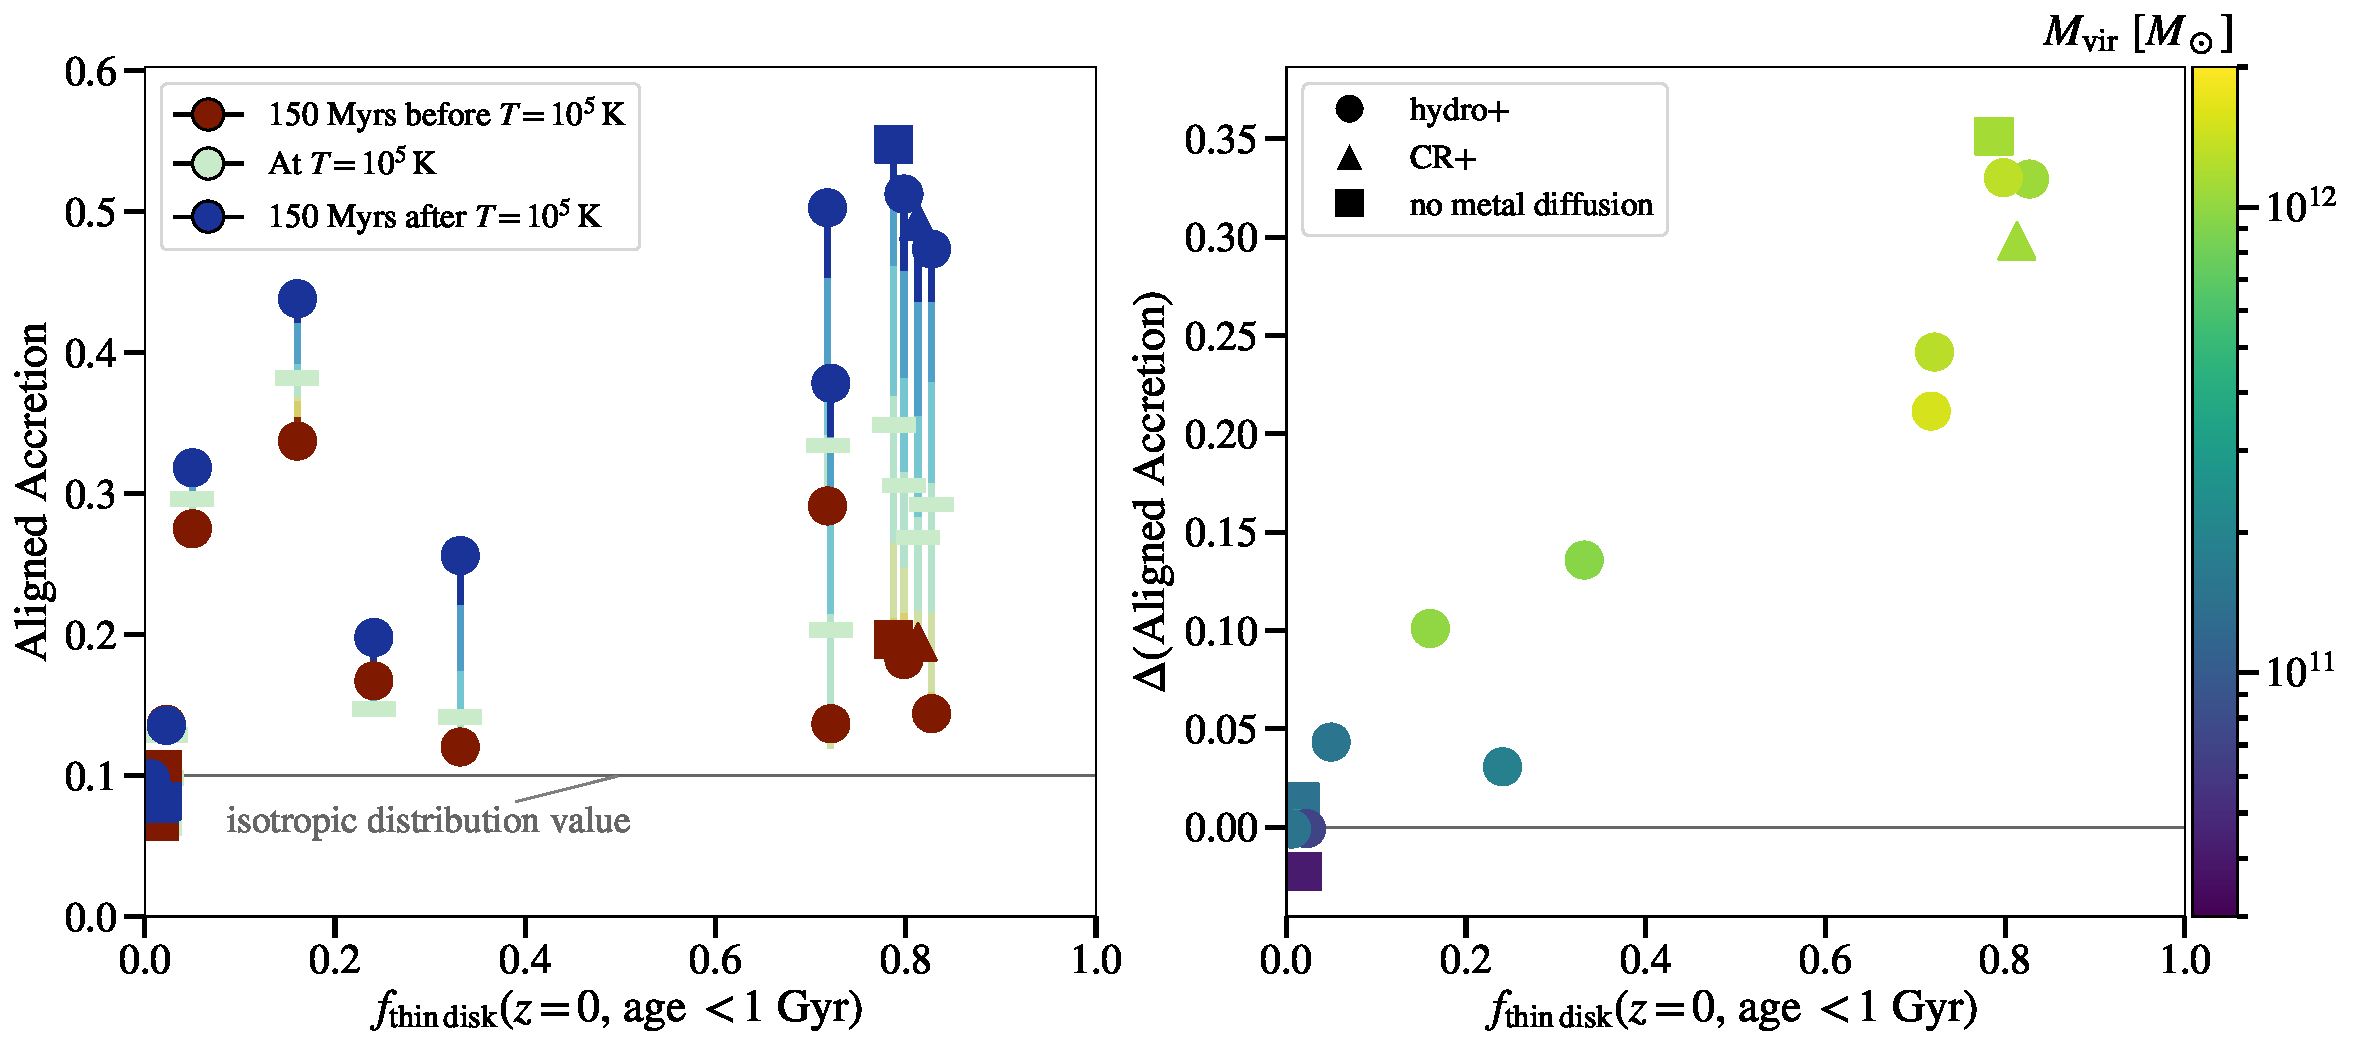
\includegraphics[width=\textwidth]{figures/prevalence/aligned_fraction.pdf}
    \caption{
    \textbf{Left:}
    Fraction of accreting mass strongly aligned ($\mid z/R \mid < 0.1$) with the disk 150 Myr before and after cooling (red and blue respectively) for our set of $\mathbf{N}$ analyzed halos.
    X-axis tracks fraction of formed within the last Gyr prior to zero that are in the thin disk ($j_z/j_c(E)>0.8$).
    Prior to cooling $\lesssim 30\%$ of accreting gas is strongly aligned with the galaxy plane,
    while after cooling that fraction increases to $\gtrsim 50\%$ for galaxies forming thin disks.
    \textbf{Right:}
    Change in aligned mass over $\pm 150$ Myr before/after accreting gas drops below $T = 10^5$ K.
    The extent to which the accreting gas changes alignment as it cools strongly tracks thin disk fraction.
    Galaxies with circularized cooling flows (quiet accretion) are in the upper right-hand corner.
    }
    \label{f: prevalence}
\end{figure*}

% PREVALENCE OF QUIET ACCRETION -- VS GALAXY PROPERTIES
\begin{figure*}
    \centering
    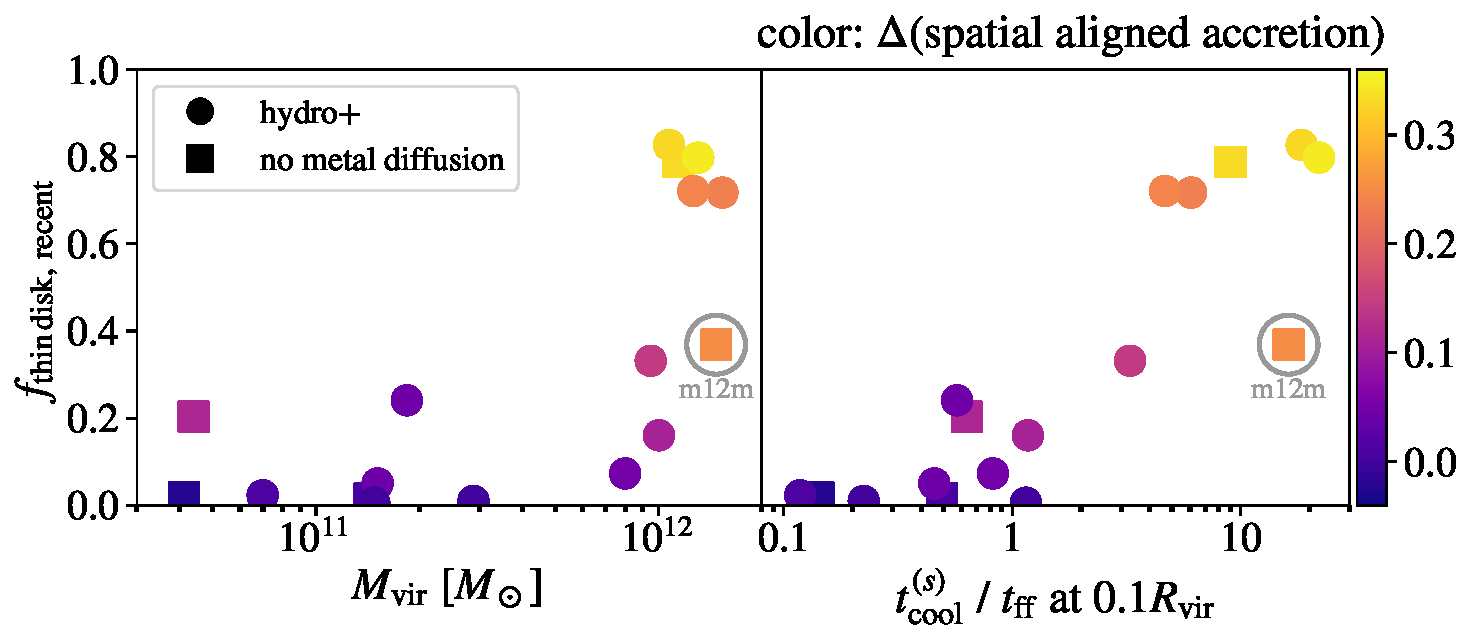
\includegraphics[width=\textwidth]{figures/prevalence/aligned_fraction_vs_galaxy_props.pdf}
    \caption{
    Change in aligned mass over $\pm 150$ Myr versus $M_{\rm vir}$ (\textbf{left}), $M_\star$ (\textbf{center}), and $t_{\rm cool}/t_{\rm ff}$ evaluated at $0.1 R_{\rm vir}$ (\textbf{right}).
    Color tracks thin disk fraction of young stars.
    $\Delta M(\mid z/R \mid<0.1)/M \sim 0$ for $M_{\rm vir} < 10^{12} M_\odot$ or $M_\star < M_{\star, {\rm MW}}$, and spans a wide range for $\sim L_\star$ galaxies.
    This demonstrates galaxy/halo mass alone is insufficient to predict accretion mode and thin disk fraction.
    The ratio of cooling time to free fall time in the inner CGM indicates the extent to which the inner CGM is in a cooling flow, and subsequently better tracks the extent to which accreting gas aligns.
    }
    \label{f: prevalence vs galaxy properties}
\end{figure*}

% % OBSERVATIONAL COMPARISON
% \begin{figure}
% \centering
% 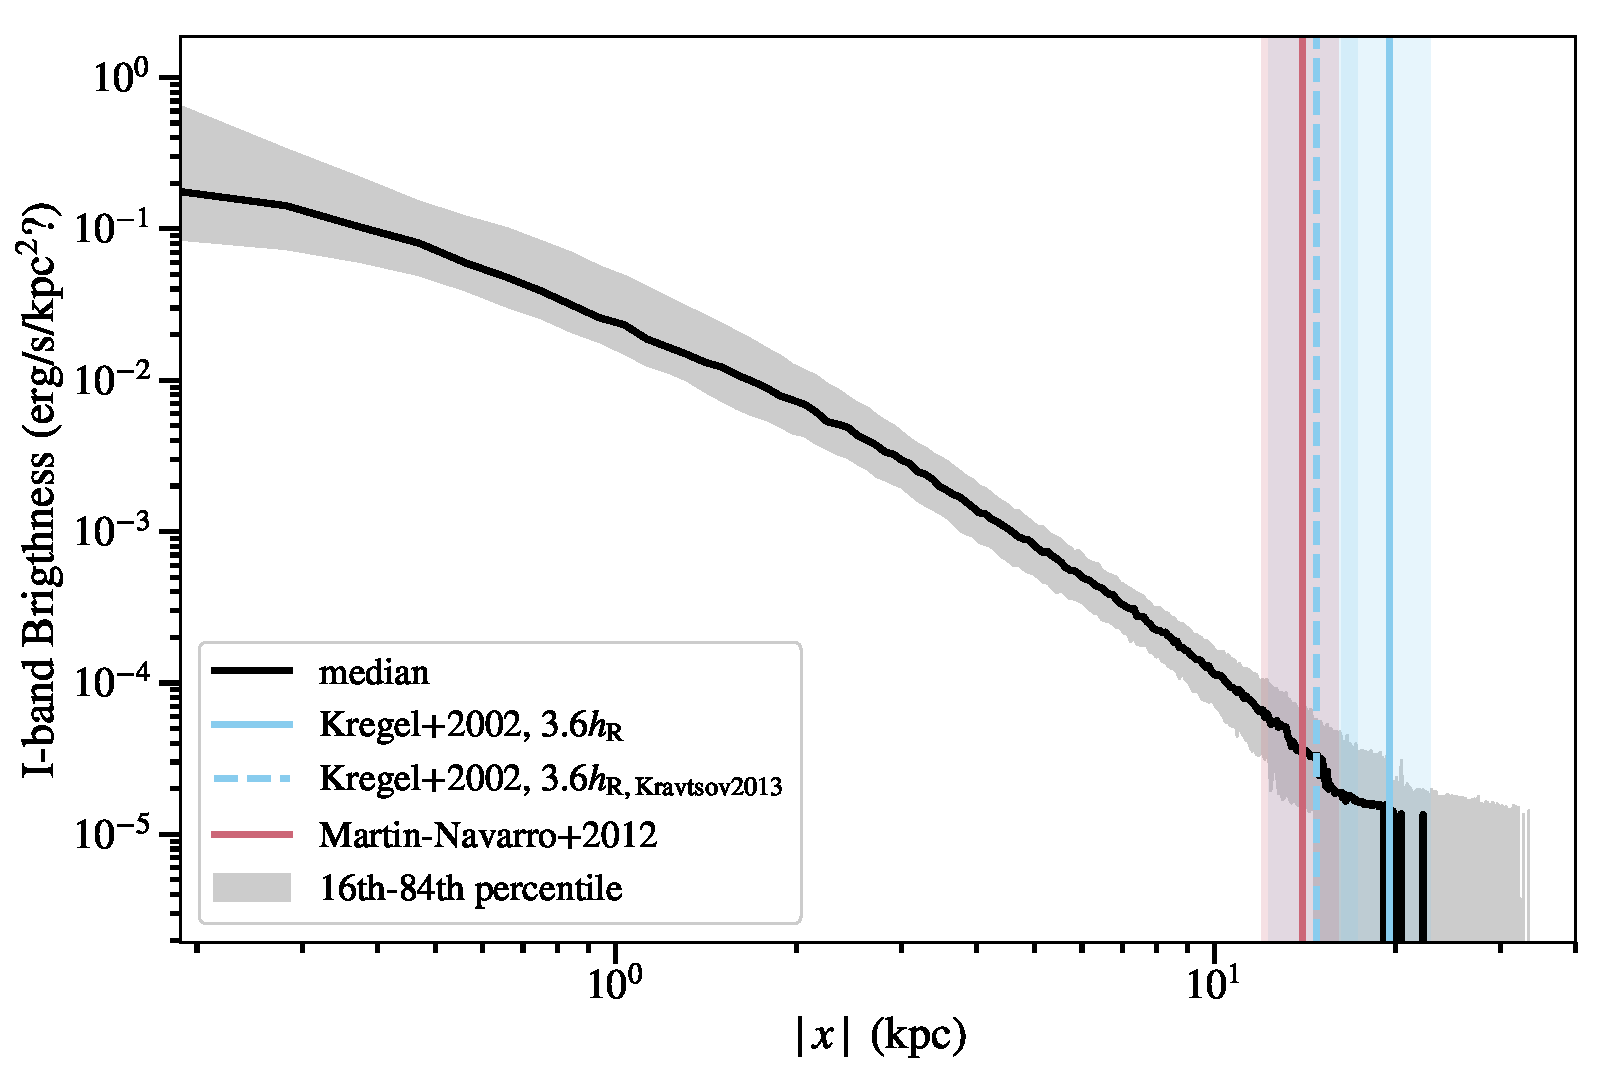
\includegraphics[width=\columnwidth]{figures/brightness_profile.pdf}
% \caption{
% I-band surface brightness profile for an edge-on stellar disk.
% Black line (shaded region) is the median (16th-84th percentile) brightness among pixels 7.5 kpc above/below the disk.
% The disk truncates at $\approx 12$ kpc, as seen by the sharp drop-off in the brightness for the percentiles, consistent with observations.
% \textbf{
% Fill out observations description.
% Put on log-linear axis.
% Cut out inner radii where dust obscuration is likely an issue.
% Maybe cut out entirely and just reference Cameron's paper.
% Reference Shea and Kareem's papers.
% }
% }
% \label{f:stellar_profile}
% \end{figure}

% SPARE FIGURE
% \begin{figure}
%     \centering
%     % \includegraphics{}
%     \caption{
%     \textbf{Spare figure, but maybe
%     cooling emission in X-ray, optical and UV lines vs.\ radius, only from tracked particles
%     }
%     }
%     \label{f: emission}
% \end{figure}

\section{NOTES FOR AUTHORS}

\subsection{KEY FOR COAUTHORS}
\textbf{Bold: Notes for things to implement.} \\
\textit{Italics: Rough text, needs polishing.} \\
Normal: Normal text, polished enough to be included in a draft.

\subsection{OUTSTANDING QUESTIONS/DISCUSSION POINTS}

\textbf{Is the weirdness with \texttt{m12i\_mhdcv} a general property of MHD sims?}
Leaving it out until I understand this.

\textbf{Change total angular momentum to that of stellar component.}

\textbf{Why is delta PDF so much better of a predictor of thin disk fraction, compared to ones that are ratio of PDF or involve the larger distribution?}
A hint is that both m12f and m12c, ones most sensitive to this, have merging galaxies $10^11 M_\odot$ halos within the last Gyr.
I think it's that Delta PDF is most-strongly correlated with quiet accretion fraction, which might predict thin disk fraction.
Next step: estimate quiet accretion fraction.
Two methods:
a) estimate peak by subtracting distribution prior to cooling.
b) particle-by-particle estimate with quiet accretion fulfilling the criteria: $j_z/j \approx 1$ within two snapshots after cooling

\textbf{How do we refer to this accretion mode?}
\textbf{Cooling flow accretion:}
Pros: Strong connection to previous work.
Cons: This accretion mode can occur in halos not undergoing cooling flows, e.g. CR halos.
Brings to mind clusters.
\textbf{Quiet accretion:}																																									
Pros: General term. Some connection to existing work, but very lightly used.
Cons: Doesn't make the connection to cooling flows clear.
\textbf{A name related to cooling flows, but not ``cooling flow accretion'':}
E.g. cooling accretion, coherent accretion, subsonic accretion.
Pros: Strong connection to cooling flow work, but isn't limited to halos with cooling flows.
Cons: Subtle changes in language can cause confusion.
\textbf{Classic hot mode:}
i.e. linking to the existing term.
Pros: Links to existing literature quite well. Reflects work that's been done.
Cons: What's new?
\textbf{Coherent cooling flow? Co-rotating cooling flow? Circularized cooling flow?}
Pros: latches on, but emphasizes difference.
Cons: relatively long.
\textbf{Some other alternative.}
Slow?
Gentle?
Spiraling?
Sharp? (Sudden and ubiquitous at angular momentum support radius.)
\textbf{Refer to it both as cooling flow accretion and quiet accretion:}
If it comes down to a choice between the two, or a technical point, refer to as a cooling flow.

\textbf{Calculate if CR and other halos are undergoing a cooling flow}
Compare inward velocity to cooling rate.

\textbf{
Which framing(s) of results to emphasize?
}
1. Accretion is an outcome of cooling flows.
2. Accretion occurs for any volume-filling, stable halo gas.
3. Accretion occurs for MW-mass halos.

% Target audience
\textbf{
Who is the target audience?
}
My thoughts are\ldots
At the broadest level anyone who wants to understand the general picture of how disks form.
Always need both theorists and observers, though a bit more focus on theorists.
Explaining a galaxy observation using CGM theory.
People who like interpretable results.

% Assess the overall message
\textbf{What points are likely to resonate with the target audience(s)?}
Imagine sitting down with the target audience.
What are the most important points you want to convey?
In particular, what could they really use?
Think first and foremost of that, and shape accordingly.

% Review
Read through the paper with each targeted group in mind.
Edit accordingly.
Even better, get a member of the target group to provide feedback.
At the end, decide on the title and the abstract.

% Citations
\textbf{I'm a bit citation-happy right now, what should I trim?}

% Temporary cooling investigation
\textbf{Why do some trajectories cool and then reheat?}
They cool because of perturbations~\citep{Esmerian2020}, but why do they reheat?
Why is there cool gas visible in the intuition-building plots 100 Myr prior to cooling?

% How much to include on CR sims
Pros of including CR-analysis:
- The physical mechanisms do not require the halo to be a classic virialized hot halo.
- According to our three characteristics that define quiet accretion, quiet accretion is observed in CR simulations.
- Quiet accretion is a more interesting concept if we point out its generality.
- Cameron Trappe also wrote a paper, and one of the main differences is the inclusion of cosmic rays. I'm not sure there's room to do a third entirely separate paper on cosmic ray quiet accretion. Most things will have been covered.
- As an extension of the previous point, because Cameron wrote the CR paper we can just include a single plot or so and point to his paper for the details of how accretion works.
Cons:
- CR halos are regarded as fundamentally different to hydro halos
- Jonathan's previous work doesn't touch on CR halos.

% Definition
Check my definition of $\tcon$.
First vs last time cooled.
Dependence on galaxy density criterion.
In Figure~\ref{f: T vs R}, as part of an ancient decision, I'm not plotting recycled material.
Is that a good choice?

% More terminology
\textbf{In regards to coherence, should we use decoherent, incoherent, or something else?}
Don't use the term coherence on its own, use dispersion of jz around the average.
\textbf{Compression heating and radiation cooling, or radiative cooling and compressive heating?}
Radiative cooling and compression heating.

% Not overly centered on disk formation
Are we overly-centered on disk formation?
Framing of conducive to disk formation might give your listeners the impression that this is the only theory for disk formation.

% Outer virialized halo effects
Check the following picture, suggested by James:
Far enough out in an m11 the inner halo is virialized, and compressive heating can contribute comparably to cooling.
This would suggest the cooling radius is max( edge of the virialized area, angular momentum radius), potentially true across all halo masses MW and below.
Can be checked by making an equivalent to Figure~\ref{f: before and after} for an m11.

% Decreasing halo mass implications
Do we want to discuss the conditions under which there could be an early onset of quiet accretion for lower-halo mass halos?

% Firefly changes
I need to set up a good preset. Requires changing using options. Can load a preset using the Options class.)
Change loading screen.
Include labels for scale.

% Plots for a future observational paper
Multi-panel image:
HI-weighted row,
OVI?-weighted row,
T-colored row.
Before column(s), at column, after column.
Try mollweide projection.
Try classic kinematic picture showing blue/red-shift along LOS.

% Additional visualizations
Try making a 2D histogram of $\Rcon$ and the angle at which it accretes.

% Angular momentum reading
There's still more angular momentum reading to be done, including:
Cadiou2020; Angular momentum evolution can be predicted from cosmological initial conditions\\
Filippo's collaborator work: \url{https://ui.adsabs.harvard.edu/abs/2017MNRAS.467..311P/abstract}\\
Krolewski2019; Alignment between filaments and galaxy spins from the {MaNGA} integral-field survey
Look at \cite{Bird2019}, which looks at alignment of galaxy disks with filaments.
Look at \cite{Bird2020}, which seems to be a typical classic disk galaxy paper.
Maller\&Dekel2002: angular momentum as a function of origin.

% Angular momentum of accreting gas vs all gas at a given radius
How does the angular momentum of all gas at a given radius compare to the angular momentum of the accreting gas?
Check by calculating the inner product between the two?

% Misaligned or warped disks
Can quiet accretion produce misaligned or warped disks?
Tjitske has seen in large scale simulations a misaligned disk being preceeded by a change in halo angular momentum.
Anna has some plots of this. This might be more present in the ELVIS sims.
The angular momentum vector of the CGM is in general misaligned with that of the stars in the central galaxy by large angles  30 to 60 degrees (DeFelippis et al. 2020).
See also Roskar2010.
Yuan Li finds changing angle of disk due to accretion in her cluster sims.

\section{Introduction}
\label{s: introduction}

% Star formation and CGM accretion
Galactic star formation is likely fueled by accretion from the circumgalactic medium (CGM), without which star formation would cease in only a couple of Gyrs~\cite[e.g.][]{Prochaska2009, Bauermeister2010, Spring2017}.
There are believed to be a number of modes of accretion from the CGM, each with different characteristics, mechanics, prevalences, and implications for star formation.
% Accretion types - hot
In the `hot' accretion mode, which has classically been associated with massive galaxies, gas first shocks to the virial temperature $\Tvir$ at the halo scale, and then radiates its gravitational and thermal energy until accreting onto the galaxy. Beyond this general framework, however, there is no consensus on the specific mechanics of hot accretion or on whether the hot gas actually manages to cool rather than being reheated by galactic feedback processes. 
% For Milky Way-analogs, theory predicts that hot gas with temperature $T>10^5$ K dominates the inflow~\citep{Faucher-Giguere2011a, VandeVoort2011, VandeVoort2012a, Joung2012, Murante2012, Nelson2013}.

One potential route for hot accretion, which has been extensively discussed in recent years, is instability-driven accretion wherein gas precipitates out of the hot halo due to thermal instabilities, forming cool clouds which lose buoyancy and accrete onto the galaxy~\citep[e.g.][]{Maller2004, Mccourt2012, Voit2015, Armillotta2016, Gronke2019a, Voit2021}.
% Quiet accretion
Alternatively, radiative cooling in the hot CGM can cause the entire hot phase to flow inward.
In this latter scenario the inward flow occurs at a rate where compressional heating of the hot phase roughly balances radiative losses, so the hot gas roughly retains its temperature.
This type of hot accretion has been discussed extensively by early studies in the context of the inner intercluster medium (ICM), where it has been termed a `cooling flow' \citep[][see \citealt{McNamara2007} for a review]{Mathews78, Cowie80, Fabian84, balbus88, Bertschinger1989}. \cite{Stern2019, Stern2020a} recently revisited these cooling flows solutions and discussed  their applicability to galaxy-scale halos.
They argued that cooling flows could be prevalent even at masses $\ll10^{12}\msun$ if halos are baryon-depleted as suggested by some theoretical and observational studies of $z\sim0$ halos \citep[e.g.,][]{Bregman2018, Hafen2019}. 

% Accretion types - cool
A third canonical accretion mode is cool, filamentary accretion, wherein cool, $T \sim 10^4$ K cosmological filaments travel into the galaxy from the IGM~\cite[e.g.][]{Keres2005, Dekel2006, Keres2009, Martin2019a}. At halo scales this mode is expected to dominate the mass inflow rate at high-redshift \citep[$z\gtrsim2$, e.g.][]{Keres2009a, Dekel2009, Huscher2020}. It is unclear however if the cool filaments remain intact down to the galaxy, or rather heat up and dissolve into the surrounding hot phase \citep{Nelson2016, Mandelker+}, in which case hot accretion onto the galaxy would be important also at high redshift. 

% Filamentary accretion can often be accompanied by ``clumpy'' accretion in the form of accreting satellite galaxies and their CGMs~\citep[e.g.][]{Hafen2019, Hafen2020}, which in some cases can fuel the formation of more than a third of the stars formed in MW-mass galaxies~\citep{Angles-Alcazar2017}.

% maybe another paragraph on other 'modes' of accretion (e.g. fountains (Oppenheimer+10) and galaxy transfer (Angles-Alcazar+17))). These modes are not really distinct from the cold/hot dichotomy, since they discuss the mass origin of the accretion, which is a different question then its thermal history and geometry which we focus on here. 

The present work focuses on hot accretion, and specifically on cooling flows where the entire hot phase is inflowing.  
From an observational perspective, cooling flows are difficult to observe for galaxies beyond
$z\sim0$~\citep{Putman2012}.
This follows since the cool CGM gas is significantly more accessible to observations than the hot CGM, but in cooling flows the accreting gas becomes cool only when it has no significant spatial or kinematic offset from the galaxy.
\citeauthor{Putman2012} thus called this accretion mode ``quiet accretion''. 
% This quiet accretion could explain observations at higher redshifts that show substantial SFRs and outflows with little, if any, evidence for accretion (e.g., Erb 2008, Steidel et al. 2010, Shapley 2011)~\citep{Putman2012}.
Consistent with quiet accretion, some observational studies argue that the accretion implied by cool gas observe in the halos of massive disks is insufficient to sustain star formation \citep{Binney09}, while others detect ionized, inflowing gas at the galaxy-halo interface~\citep{Zheng2017}. 

% Previous idealized simulations have studied cool gas clouds condensing onto galaxies and found that disrupted and heated clouds could condense and cool at disk edge~\citep{Heitsch2009}.
% However, to-date little work has been done to determine how prevalent quiet accretion is in a cosmological environment, as well as the detailed mechanics of how it proceeds.

% \citep{Miller16}

% Cosmological simulations
Modern cosmological simulations provide a means to understand the prevalence, mechanics, and characteristics of the different accretion modes.
These simulations include a combination of cosmological environment and galactic physics, which has allowed simulators to investigate accretion while accounting for both its cosmological nature and its interaction with galaxies and their CGM~\citep[e.g.][]{Oppenheimer2010, Stewart2011, Fernandez2012, Ford2014, Angles-Alcazar2017, Hafen2019, Hafen2020, Ho2019, Rottgers2020, Trapp2021}.
Of special note are ``zoom-in'' simulations that focus on resolving a single halo and its environment, enabling high resolution while preserving cosmological structure~\citep[e.g.][]{Katz1993, Hopkins2014, Hopkins2018, Wang2015, Agertz2020}.
Among these the FIRE simulations~\citep{Hopkins2014, Hopkins2017}\footnote{\url{https://fire.northwestern.edu/}} are a set of zoom-in simulations that resolve stellar feedback on the scale of giant molecular clouds in the ISM, producing winds that naturally expand into the CGM and interact with accreting gas~\citep{Muratov2015, Muratov2017, Hafen2019, Hafen2020}.
The resultant galaxies are broadly consistent with the stellar mass-halo mass relation~\citep{Hopkins2017}, the mass-metallicity relation~\citep{Ma2016a}, satellite galaxy populations~\citep{Wetzel2016, Garrison-Kimmel2019a}, and can have thin-disks consistent with Milky Way-like galaxies~\citep{Garrison-Kimmel2018, El-Badry2018}.

In this paper we demonstrate that cooling flows (or `quiet accretion') is the primary mode of gas accretion onto central Milky Way-mass galaxies at $z \sim 0$ in the FIRE simulations. 
We utilize the 3D nature of the simulations to explore the mechanics of quiet accretion near the disc-halo interface, thus going beyond the 1D steady-state solutions developed in classic ICM studies, and extending the idealized 3D simulations in \cite{Stern2020} to a more realistic cosmological setting. 
% Our simulations include stellar feedback processes but no AGN feedback processes, this result suggests that cooling flows may be  prevalent in galaxies where AGN feedback is weak or absent, and that cooling flows can be used as a benchmark for AGN feedback studies. 

% This paper
This paper is structured as follows. 
In \S\ref{s: methods} we describe our simulation sample and primary sample of particles selcted from the simulations.
In \S\ref{s: characteristics} and \S\ref{s: prevalence} we show that the vast majority of accreting gas has characteristics consistent with quiet accretion.
In \S\ref{s: mechanics} we analyze the mechanics through which quiet accretion occurs.
In \S\ref{s: broader prevalence} we discuss the prevalence of the quiet accretion mode, focusing on the conditions that enable quiet accretion, including an equivalent mode in halos with non-thermal support.
In \S\ref{s: modes} we compare quiet accretion as seen in our simulations to other accretion modes.
In \S\ref{s: fueling} and \S\ref{s: disk formation} we discuss the implications of quiet accretion for fueling star formation and encouraging disk formation, respectively.
We conclude in \S\ref{s: conclusions}.
% We offer some brief insight on observational expectations for quiet accretion in \S\ref{s: observational expectations} before concluding in \S\ref{s: conclusions}.

% % Observational evidence
% \textbf{
% Reaches back to Barcons+1995: https://www.nature.com/articles/376321a0.
% See also Yong+2017ab.
% \url{https://ui.adsabs.harvard.edu/abs/1995Natur.376..321B/abstract}
% \url{https://ui.adsabs.harvard.edu/abs/2013Sci...341...50B/abstract}
% \url{https://ui.adsabs.harvard.edu/abs/2016ApJ...820..121B/abstract}
% \url{https://ui.adsabs.harvard.edu/abs/2019MNRAS.485.1961Z/abstract}
% \url{https://ui.adsabs.harvard.edu/abs/2017ApJ...835..267H/abstract}
% Bielby et al. 2017; Péroux et al. 2017; Diamond-Stanic et al. 2016; Muzahid et al. 2016
% Wong et al., 2004; Martin et al., 2012; Rubin et al., 2012; Ho \& Martin, 2020
% Zabl 2019
% Zheng2017
% }

% % C-A comments
% \textbf{
% Galaxies have lower j than the CGM due to preferential accretion of low-j gas.
% Low angular momentum gas is more likely to form stars because it moves inwards and increases density.
% https://ui.adsabs.harvard.edu/abs/2019MNRAS.488.4801J/abstract
% https://ui.adsabs.harvard.edu/abs/2015MNRAS.449.2087D/abstract
% this paper also discusses/assumes low sAM gas preferentially ends up in stars:
% https://ui.adsabs.harvard.edu/abs/2017MNRAS.466.1625Z/abstract
% }

% Jonathan Info dump
% Some refs on truncation radius in observations:
% \cite{Kregel2002} tight correlation between disk truncation radius and Re (Spearman 0.95) in 34 edge-on spirals (in face-on galaxies stellar halos can outshine truncation, see Martín-Navarro+14). $R_{\rm truncation} / R_e({\rm Iband}) \sim~ 3.6$. Somewhat higher ratio in small Re spirals, somewhat lower ratio in bluer passbands (where Re is larger).
% Re is independently found to be proportional to the virial radius, roughly Re ~ 0.015 Rvir (e.g. Kravtsov13).
% Martín-Navarro+12: 34 edge-on spirals from SDSS / S4G: Rtruncation ~ 1.1 R25, where R25 is the radius at which the surface brightness equals 25mag
% van der Kruit+07: when a HI-warp is present in the gaseous disc it starts at 1.1 Rtrunc; the truncation radius and the onset of the warps coincide radially sometimes with features in the rotation curve and often with steep declines in the HI surface density; inner disks are very flat and the onset of the warp just beyond the truncation radius is abrupt and discontinuous;
% Perez+04, Trujillo\&Pohlen05, Azzollini+08: measurements of truncation radius at z~1
% Comeron+12: 70 edge-on S4G galaxies. 77\% of thin discs truncate, but only 31\% of thick discs. $M_thick/M_thin$ increases with decreasing $v_c$
% de Jong+07: Stellar Populations across the NGC 4244 Truncated Galactic Disk
% Haberzettl+07: truncation in LSBs
% some suggested theoretical explanations of breaks:
% https://ui.adsabs.harvard.edu/abs/2009MNRAS.398..591S/abstract
% https://ui.adsabs.harvard.edu/abs/2008ApJ...675L..65R/abstract
% https://ui.adsabs.harvard.edu/abs/2006ApJ...645..209D/abstract
% https://ui.adsabs.harvard.edu/abs/2009ApJ...705L.133M/abstract
% https://ui.adsabs.harvard.edu/abs/1987A%26A...173...59V/abstract
% and short summary sentence from Comeron+12 intro:
% "Several theories compete for explaining the origin of such breaks. Truncations have been explained by dynamical arguments related to the conservation of angular momentum during galaxy formation, by star formation thresholds, and by the redistribution of angular momentum by a bar. Antitruncations have in some cases been linked to interactions and mergers."
% Antitruncations are cases where the Surface Brightness profiles flattens at large disc radii rather than steepens. From my impression of the observational literature anti-truncations are seen mainly in face-on galaxies and are related to the existence of stellar halos

% \textbf{
% Misc notes from Halo21
% Norbert Werner sees the X-ray atmosphere is flattened, along the disk.
% Mark Voit: complementary view is that rotation destabilizes halo gas.
% Sormani and Serbachi idealized rotating hot halos.
% Oppenheimer rotating hot halo.
% }

% % Observational inflow evidence
% \textbf{
% Hwang, Barrera-Ballesteros, Heckman+2019: ``anomalously low-metallicity regions'' in MaNGA galaxies in $\sim 25\%$ of MaNGA SF galaxies. Luo, Heckman+2021 is a follow-up.
% Howk, Rueff, Lehner+2018: extraplanar gas is lower metallicity.
% Putman, Peek,\& Joung 2012, Putman review for HVCs, best fit inflow speeds are -40 km/s, predict accretion rate of $\sim 0.1 M_\odot/$ year (with correction factor multiplied by two for ionized component; Lehner\&Howk 2011).
% IVCs: Rubin+2019 is a good start, Richter+2017 provides a review.
% Bregman hot halo rotation (cited by Ben).
% }

% % Radial Inflow
% \textbf{
% Observational estimates of disk rotation:
% https://ui.adsabs.harvard.edu/abs/2004ApJ...605..183W/abstract
% https://ui.adsabs.harvard.edu/abs/2019ApJ...883...77S/abstract
% }

% \textbf{Just go through Crystal Martin's Halo21 Keynote...}

% \textbf{The accretion isn't completely polar symmetric.}

% \textbf{Galaxy size and relation to angular momentum:
% https://ui.adsabs.harvard.edu/abs/2017rlbc.confE..29K/abstract}

\section{Methods}
\label{s: methods}

\subsubsection{Simulation sample}
\label{s: methods -- simulations}

% Simulation sample
\textbf{We need to decide what galaxies to include, after which I'll fill this out.}
\textbf{Also do massive galaxies?}

% Comparable samples
\textit{
\cite{Garrison-Kimmel2018} perform a related analysis using simulations from the ELVIS suite and \texttt{m12i\_md}, \texttt{m12f\_md}, \texttt{m12b\_md}, \texttt{m12m\_md}, \texttt{m12c\_md}, \texttt{m12w\_md}, \texttt{m12q}, \texttt{m12z\_md}.
\cite{Yu2021} perform a related analysis using simulations from the ELVIS suite and \texttt{m12i\_md}, \texttt{m12f\_md}, \texttt{m12b\_md}, \texttt{m12m\_md}, \texttt{m12c\_md}, and \texttt{m12w\_md}.
Gurvich et al., in prep, perform a related analysis using simulations \texttt{m12i\_md}, \texttt{m12f\_md}, and \texttt{m12b\_md}.
}

\textbf{Table should include $n_{\rm particles}$ in the sample.}

% Metal diffusion
The metal distribution in the CGM affects cooling processes and therefore the treatment of metal diffusion is important for resolving substructure and small clouds~\cite{rennehan2021}.
More diffusive metal diffusion typically produces fewer cool clouds, with possible exceptions for stripping processes, and many current prescriptions for metal diffusion may under-resolve metal diffusion~\citep[e.g.][]{rennehan2019, rennehan2021}.
Therefore if cool cloud substructure is not present with under-resolved metal diffusion, as may be the case in our simulations, we do not expect it to arise with an alternative treatment.

\subsubsection{Analysis}
\label{s: methods -- analysis}

\textbf{Mention minInd.}

% How we select the particles
For a given galaxy we select all resolution elements (particles) that are in the central galaxy at $z=0$ and in the CGM 1 Gyr prior.
The galaxy is defined as all gas and stars inside $R_{\rm gal}$, with an additional density cut of $n_{\rm H} = 0.13$ cm$^{-3}$ for gas.
For $R_{\rm gal}$ we use the same tested definition as \cite{Hafen2019, Hafen2020} of $R_{\rm gal} = 4 R_{\star,0.5}$.
The CGM is defined as all gas inside $0.1 -1 R_{\rm vir}$.
For each selected particle we retrieve the full history of the particle (including temperature, density, metallicity).

% Handling duplicate IDS
Of the particles targeted to be tracked $<2\%$ are particles that will accumulate or have accumulated at least twice their mass' worth in deposited mass from stellar feedback, resulting in them being split into two particles.
These particles pose a problem for tracking because the history of the additional mass is not recorded and likely comes from a variety of sources.
As done in previous particle-tracking analyses~\citep{Hafen2019, Hafen2020}, we discard these particles, which are not expected to affect our results due to their small contribution.

% Definition of t1e5 and calculating it
A key time for our analysis is the last time each particles transitions from $T > 10^5$ K to $T< 10^5$ K, referred to as $\tcon$.
For gas that cools as it accretes, $\tcon$ occurs as the gas passes through the galaxy-halo interface.
When selecting values in the simulation corresponding to $\tcon$ we use the last snapshot an accreted particle had $T > 10^5$ K, i.e. the snapshot immediately before the transition.
Note that we do not account for gas particles being heated to $T > 10^5$ K while still in the ISM.
Because our sample of tracked particles focuses on recently accreted particles this is expected to be a small population that will not contaminate our analysis.
This is confirmed a posteriori in Figure~\ref{f: theta vs t}, where gas is not preferentially oriented in a disky ISM prior to $\tcon$.

\section{Results}
\label{s: results}

% This section will describe results

\subsection{How do MW-like galaxies accrete?}
\label{s: characteristics}

% Summary picture description
To characterize gas accretion we analyze the central galaxy and its CGM from $z=0$ to one Gyr prior.
Figure~\ref{f: overview} shows three example trajectories of how gas accretes onto MW-mass galaxies, selected as described in \S\ref{s: methods}.
Tracks are shown for \texttt{m12i}.
Gas moves inwards with a temperature $T \sim T_{\rm vir} \sim 10^{5.5}$ K, cools at the galaxy-halo interface, and aligns with the galaxy as it cools.
We show in the following sections (\S\ref{s: characteristics -- inflowing gas phase}--\ref{s: characteristics -- aligns}) that these are the primary characteristics of gas accretion onto our simulated MW-mass galaxies.
% We define gas accretion with these characteristics as \textit{quiet accretion}~(\S\ref{s: characteristics -- definition}).

\subsubsection{Hot inflow through the CGM}
\label{s: characteristics -- inflowing gas phase}

% Intro and figure description
We first determine if accretion in the inner halo is dominated by hot or cold flows of gas.
Figure~\ref{f: Mdot} shows the mass inflow rate of different gas phases at a given radius in two of our simulated halos.
Mass flow rates are the average over the course of one Gyr, ending at $z=0$.
We calculate the mass inflow rate as
\begin{equation}
     \Mdot = \frac{\int_{\rm shell} v_r dm}{\Delta r} = \frac{M_{\rm shell}}{\Delta r} \langle v_r\rangle_{\rm mass\, weighted}
     \label{e: Mdot}
\end{equation}
where $\Delta r=0.05\,{\rm dex}$ is the shell thickness, and the integration is done on all particles with centers within the shell.

% Consequences
The inwards mass flux of hot CGM gas (red curve; $T>10^5$ K)  is $\gtrsim 4\times$ that of the cool CGM gas (blue curves; $T < 10^5\,{\rm K}$) down to $r \approx 20-30$ kpc.
% The greater mass flux of hot gas suggests hot mode accretion is the dominant form of accretion in our halos.
The greater mass flux of hot gas indicates that \textit{the dominant form of accretion in our halos is an inflowing hot phase}, rather than cold flows or cool clouds precipitating from the hot phase. 

The radius of $\approx 20$ kpc where the hot inflow rate drops is the edge of galactic star formation, as shown by the flattening of the enclosed star formation rate~($\dot M_{\rm stars}(<R)$; black dashed curve), and the radius where angular momentum support in the hot gas becomes significant, as shown below. 
Note also that the inwards mass flux of all gas (top panel) as well as all hot gas is approximately constant down to $\approx 20$ kpc.
The constant mass flow across radii indicates gas in the inner halo is roughly in a steady state, similar to the assumption of cooling flow solutions~\citep{Stern2019}.

\textbf{$\dot{M}_{\rm stars}$ in Fig.~\ref{f: Mdot} is currently SFR$/2$. Change to SFR minus gas returned from winds/SNe.}

\subsubsection{Cools at the galaxy-halo interface}
\label{s: characteristics -- cools}

\textbf{Mention that we don't show particles ejected from the galaxy.}

% Rcon
A key quantity for differentiating modes of hot accretion is the radius at which gas last cools before accreting onto the galaxy, i.e. the radius at time $\tcon$, $\Rcon \equiv R (\tcon)$.
For gas that cools in the halo and subsequently precipitates $\Rcon$ will be at CGM scales, while for a cooling flow we expect $\Rcon$ to be at the galaxy-halo interface.
The top panels of Figure~\ref{f: T vs R} show the distribution of $\Rcon$ for two MW-like galaxies at $z\sim0$.
All particles with $\Rcon>100$ kpc were placed at $R=100$ kpc bin. 
The distribution peaks just outside the galaxy edge, with a median of $\Rcon \approx 0.06 R_{\rm vir}$ and only xx\%\ of particles cooling beyond $\sim 40$ kpc.
This result is consistent with cooling flows and quiet accretion, and inconsistent with a precipitation scenario where clouds cool far in the halo and subsequently accrete.
% By comparison, isotropic cooling occurring randomly within $R_{\rm vir}$ would cool in a wide distribution with a median at $0.8 R_{\rm vir}$, while for our accreted gas 

% Accretion tracks figure description
The bottom panels of Figure~\ref{f: T vs R} show the temperature and radial history of 5 randomly-selected accreted particles.
These particles typically have $T>10^5$ K, with only temporary periods of cooling to lower temperatures.
% Nevertheless, the temperature-distance trajectories through the hot halo are highly variable, including times where gas can cool to $T \sim 10^4$ K.
Previous work shows that such cooling events are typically the result of perturbations in the CGM, usually from satellite galaxies and their CGMs~\citep{Esmerian2020}.
These cool condensations however typically heat up and rejoin the hot phase prior to accreting onto the galaxy. 

\subsubsection{Cooling is simultaneous with circularization}
\label{s: characteristics -- aligns}

% Figure description/introduction
Figure~\ref{f: theta vs t} plots the geometry of accreting gas at different times relative to $\tcon$.
Times prior to cooling are colored in red, while times after cooling are plotted in blue.
The curves shows the PDF of $\cos \theta$, where $\theta$ is defined as the angle between the gas element position and the total angular momentum vector of the stars inside the galaxy.
A spherical distribution of accreted gas would have a flat pdf with a value of 0.5, while 
the pdf of accretion in the disc plane would be a delta function centered at $\cos\theta = 0$.
The plot shows that gas accreting onto $\sim L^\star$ FIRE galaxies transitions from being distributed quasi-spherically prior to cooling to being distributed in the galaxy plane after cooling, over $\lesssim 200$ Myr.
This indicates that cooling and circularization of the accreted gas occurs simultaneously, as suggested also by 1D cooling flow solutions \citep{Stern2020}. 

% \subsubsection{Quiet accretion}
% \label{s: characteristics -- definition}

% The characteristics highlighted in \S\ref{s: characteristics -- inflowing gas phase} to \S\ref{s: characteristics -- aligns} are the primary characteristics of \textit{quiet accretion}:
% \begin{enumerate}
%     \item The accreting gas is predominantly hot ($T \sim T_{\rm vir}$) from $R_{\rm vir}$ down to the galaxy-halo interface~(\S\ref{s: characteristics -- inflowing gas phase}).
%     \item The accreting gas rapidly cools to $T \sim 10^4$ K at the galaxy-halo interface~(\S\ref{s: characteristics -- cools}).
%     \item The accreting gas forms a coherent disk as it cools, prior to which it is distributed quasi-spherically~(\S\ref{s: characteristics -- aligns}).
% \end{enumerate}

% Notes on the name
% Hot accreting gas that cools and accretes at the galaxy-halo interface has previously been termed \textit{quiet accretion}~\citep{Putman2012}.
% The name ``quiet accretion'' reflects both the challenge in detecting the hot, low-density gas prior to cooling (\textbf{Good citations for this?}), and the ``soft-landing'' of the coherent disk gas onto the galaxy (more in \S\ref{s: disk formation}).

% Notes on the definition
% Two aspects of the definition:
% First, while quiet accretion should be predominantly hot down to the galaxy-halo interface, temporary cooling can occur, as is demonstrated for some trajectories in Figure~\ref{f: T vs R}.
% Importantly, cooling in the halo (as opposed to near the galaxy-halo interface) is not predictive of whether or not the gas will accrete onto the galaxy~\citep{Esmerian2020}.
% This allows us to separate this temporary behavior from our definition of quiet accretion.
% Second, while the accreting gas should form a coherent disk as it cools, our definition does not require it to be aligned with the galaxy.
% Quiet accretion may still occur for halos with angular momentum significantly misaligned with the galaxy, and analysis of cosmological simulations suggests that misaligned CGMs can produce warped, misaligned, or counter-rotating disks~\citep[e.g.][]{Roskar2010, Starkenburg2019}.

\textbf{Move the commented out above to the summary, and condense.}

\subsection{Mechanics of cooling flows at the galaxy-halo interface}
\label{s: mechanics}

% Figure description
In this section we examine the mechanics responsible for the trajectories and properties of accretion onto MW-mass halos.
Figure~\ref{f: before and after} shows a selection of properties for each accreted gas element as a function of time relative to cooling  ($t - \tcon$; \S\ref{s: methods}).
% Figure~\ref{f: before and after} demonstrates that gas cools (A; temperature vs time) and stalls at the galaxy edge (B; radius vs time) because it becomes fully angular-momentum supported (C; ratio of angular momentum vs time), by which time it is rotating coherently in the same direction (D; fraction of angular momentum aligned with galaxy), allowing the gas to quickly collapse into a disk when the cooling exceeds the heating (E; change in specific energy).
The properties of particles at each $t - \tcon$ are binned together and used to calculate the median of the property (black line) and its 16th to 84th percentile range (shaded region).
We now go through each panel in detail.

\subsubsection{Inflowing and hot to stalled and cool}
\label{s: mechanics -- temp and radius}
Panels (A) and (B) in Figure~\ref{f: before and after} respectively show gas temperature and radius at a given time relative to the final cooling time.
% By definition, gas last cools at $t=\tcon$. 
The temperature panel shows that the distribution of accreted gas temperatures are practically disjoint prior and post the last cooling time, with $80\%$ of particles having $T > 10^5$~K prior to last cooling, in contrast with the gas temperature spanning $\sim100- 10^4$ K after cooling. 
The radius panel demonstrates that last cooling occurs at $R_{\rm gal}$ (defined to enclose the $\sim90\%$ of the stellar mass), consistent with the result of  Figures~1-4.
At earlier times the accreted gas is inflowing, traversing the inner 50 kpc of the halo within $\approx500$ Myr, corresponding to an average inflow velocity of $v_r\approx-100$ km s$^{-1}$.
This radial velocity is smaller than the characteristic circular velocity of 200 km s$^{-1}$ in these halos, suggesting significant pressure support $(\approx1-(v_r/v_c)^2\approx75\%)$ as expected for a hot inflow.
After reaching $R_{\rm gal}$ the inflow almost entirely stalls, and proceeds within the disc at a significantly slower velocity of $xx$ km s$^{-1}$ (ref Trapp's paper). 
% showing behavior characteristic of quiet accretion.

\subsubsection{Angular momentum support and coherence}
\label{s: mechanics -- angular momentum}

% Support
Figure~\ref{f: before and after}, panel (C) shows the magnitude of the specific angular momentum ($\mid \vec j \mid = \mid \vec r \times \vec v \mid$; green) and the z-component of the specific angular momentum ($j_z$; purple).
The z-direction is defined as parallel to the net angular momentum of stars within $R_{\rm gal}$.
The median $j_z$ is equal to $\approx 2500$ kpc km s$^{-1}$, comparable to the average specific angular momentum of $\lambda \vvir \Rvir=\mathbf{xx}\lambda_{0.035}$ expected in dark matter halos due to tidal torques (\cite{Rodriguez2016}, where $\lambda = 0.035 \lambda_{0.035}$ is the spin parameter,  $\Rvir=zz$ is the virial radius, and $\vvir$ is the virial velocity).
The panel further demonstrates that the value of $j_z$ is practically constant prior to accretion, indicating the inflow conserves angular momentum in this direction.
For comparison, the dashed line plots the specific angular momentum necessary for gas to be fully supported by angular momentum at a given radius, i.e. $Rv_c(R)$.
The two curves converge shortly after $t=\tcon$, again indicating the cooling and a transition to rotational support occur almost simultaneously. 

% Coherence
% As the gas gains support it also becomes more coherent.
Panel C also shows that $\mid \vec j \mid$ decreases prior to cooling, from $\approx 5000$ kpc km s$^{-1}$ to $\approx 3000\,{\rm kpc\,km s}^{-1}$, in contrast with  $j_z$ which remains constant.
This trend is explored in  panel (D), which shows the distribution in the ratio $j_z/\mid\vec j\mid$ of accreting gas.
% Gas is rotating parallel to the galaxy if $j_z/\mid \vec j \mid=1$, while $j_z/\mid \vec j \mid=0$ signals perpendicular rotation and $j_z/\mid \vec j \mid=-1$ signals counter-rotation.
The width of the distribution (as shown by the shaded region) indicates the rotational coherence of the gas. 
%, regardless of its alignment with the disk.
At $t-\tcon=-500$ Myr the ratio $j_z/\mid\vec j\mid$ spans a large range of $\approx -0.3 - 0.9$ (negative values indicate counter-rotation).
% , i.e. ranging from rotation perpendicular to the galaxy to nearly fully-aligned, with the 16th to 84th percentile interval spanning $\sim 0.3$.
By $\tcon$ nearly all the accreting gas has $j_z\approx\mid\vec j\mid$, indicating all hot accreting gas particles are co-rotating. 
These trends suggest that components unaligned with the net angular momentum are canceling each other out due to interaction in the hot halo, as found also by other cosmological simulations ~\citep[e.g.][]{DeFelippis2017}.
% From $t-\tcon = 500$ Myr to $t=\tcon$ the j_zmagnitude of specific angular momentum for individual particles decreases 
% However, This increasing rotational support with decreasing radius is responsible for the stalling seen in panel (B), and is a feature of many simulations of $L^*$ halos~\citep[][]{Oppenheimer2018}.
The result that the hot halo just outside the galaxy is co-rotating with the galaxy is also consistent with recent kinematic analyses of hot gas in the Milky-Way halo \citep{Miller2016}. 

% The angular momentum increase
There is small-but-noticeable increase in the specific angular momentum of each gas particle at $t \approx \tcon$.
This increase is not the focus of our analysis, but we note that it may be a result of a difference in orientation and/or amplitude between the angular momentum of the galaxy and the angular momentum of the accreting gas~\citep[e.g.][]{Danovich2012, DeFelippis2017, DeFelippis2020}, which forces the accreting gas to co-rotate with the galaxy, as hinted at by the larger increase in $j_z$ compared to $\mid \vec j \mid$.
The explicit mechanism to increase $j_z$ may be exchange of angular momentum via gravitational torques~\citep[e.g.][]{Danovich2015} or via collisional interactions.
Any angular momentum gained is expected to be lost by other particles, driving inflow of existing gas particles in the galaxy or galaxy-halo interface.

% Distribution of R1e5
Comparison between panel (C) and panel (D) reveals the origin of the spread in $\Rcon$ values seen per halo in \S\ref{s: characteristics -- cools}:
there is a range of specific angular momentum values spanning $\mid\vec j\mid \sim$, but in all cases $\mid\vec j\mid = j_z$ after cooling.
The range in specific angular momentum values sets a range in radii at which gas stalls and cools, while still becoming fully aligned with the disk.
\textbf{
This point might need a separate figure if we really want to include it.
}

% \textbf{Do we want to add some discussion here on how the gas gets its angular momentum from the IGM, i.e. tidal torque theory?}

\subsubsection{Support leads to cooling}
\label{s: mechanics -- energy balance}

% Energy balance description
In Figure~\ref{f: before and after} panel (E) we assess the energetics of the gas to determine why it cools.
We study the energetics through two types of change in specific energy: radiative cooling (blue lines) and compressive heating (red lines).
Radiative cooling per unit mass for an individual particle is calculated as $\nH^2 \Lambda / \rho$, where $\nH$ is the Hydrogen density, $\rho$ is the mass density, and $\Lambda$ is the cooling function, which we take from \cite{Wiersma2009a}.
Compressive heating per unit mass for an individual particle is calculated as $P \frac{dV}{dt} \approx \frac{ P }{ \rho^2 } \frac{ \Delta \rho }{ \Delta t }$, where $P = n k_B T$, $\Delta \rho$ is the change in density from one snapshot to the next, and $\Delta t$ is the typical snapshot time spacing.
Because accreting gas elements interact with other accreting gas elements thermodynamically we show the mean specific energy tracks of all gas elements binned into 100 Myr bins of $\tcon$.
To avoid outliers with artificially-large heating or cooling rates affecting the results we discard the $1\%$ of particles with highest change in specific energy.
Some $\tcon$ bins contain much more accreting gas than others, and to reflect this we set the darkness of the lines proportional to the number of particles in the bin.

% Energy balance trend
Prior to $\tcon$ radiative cooling increases by a factor of $\sim 10$ over the course of 500 Myr, from 0.01 erg s$^{-1}$ g$^{-1}$ (corresponding to a cooling time of \textbf{xx}) to 0.1 erg s$^{-1}$ g$^{-1}$ (corresponding to a cooling time of \textbf{yy}).
The radiative cooling is however nearly completely offset by compressive heating, consistent with the roughly flat temperature profile shown in Panel (A).
This equality of radiative cooling and compressive heating is a defining characteristic of cooling flows \citep{Mathews78, McNamara2007, Stern20}. 

At $t=\tcon$ the cooling rate increases sharply, a result of increased density from gas piling up at the angular momentum support radius (as also seen in \citealt{Trapp2021}).
At roughly the same time compressive heating drops off dramatically due to the lack of inward movement.
The result is gas that cools over the course of $\lesssim 50$ Myr.

\textbf{
Add diagnostic panel showing density.
}

\textbf{
How am I treating 1e4 K gas?
As radiatively cooling, or in UVB equilibrium?
}

% This is old stuff Jonathan wrote. Keeping around for now.
% To demonstrate that the hot radial inflow is driven by cooling, we compare the different terms of the energy conservation equation. In steady-state, and assuming the gravitational potential is constant,  energy conservation in the radial direction dictates \citep[e.g.][]{Shu82}
% \begin{equation}\label{e: energy}
%     \rho g v_r + H_{\rm feedback} - \frac{d}{dr}(v_r P)= 
%     \frac{d}{dr}\left(\rho v_r \left(\epsilon+\frac{1}{2}v^2\right)\right)  +  \nH^2\Lambda  
% \end{equation}
% where the terms on the left hand side are the `source terms' -- gravity, feedback, and the work done on the shell by adjacent shells, while the terms on the right represent respectively the heating and acceleration of the flow and radiative losses. 
% Integrating over radial shells and rearranging we get the energy integral
% \begin{equation}
%     \Mdot\frac{d}{dr}\left(\Phi+\frac{3}{2}\epsilon + \frac{1}{2}v^2\right) = 4\pi r^2 \left(\langle\nH^2\Lambda\rangle-\langle H_{\rm feedback}\rangle\right)
% \end{equation}
% In Fig.~\ref{f: Edot} we plot each of the terms in eqn.~(\ref{e: energy}), averaged over radial shells and over time. Shell averages of quantity $Q$ are calculated via 
% \begin{equation}
%     \frac{d\dot{E}_Q}{d r} = \frac{\int_{\rm shell} Q\rho^{-1} dm}{\Delta r} 
% \end{equation}
% where the intergral is over all particles within the shell and $\Delta r$ is the thickness of the shell. The factor $\rho^{-1}$ is since eqn.~\ref{e: energy} is in Eulerian form. We then take the average of all shells at a given $r$ in snapshots of the last Gyr of the simulation. 
% In order to calculate the compression term from a single snapshot, we make the following further approximation \textbf{(TBD: check if justified)}
% \begin{equation}
%     \frac{d\dot{E}_{\rm comp}}{d r} \approx 
%     \Mdot P \left\langle\frac{d V}{d r}\right\rangle_{\rho v_r} \approx
%     \Mdot P \frac{d\langle V \rangle_{\rho v_r} }{dr}
% \end{equation}
% Note that since $d\ln\rho/ d\ln r$ is of order unity, and in hot virial temperature gas $\epsilon/r \approx c_{\rm s}^2/r \approx v_{\rm c}^2/r = g$, we get that $\dot{E}_{\rm comp}$ (eqn.~\ref{e: Ecomp}) and $\dot{E}_{\rm grav}$ (eqn.~\ref{e: Egrav}) are of the same order.

\subsection{Prevalence of quiet accretion}
\label{s: prevalence}

% Figure description
Figure~\ref{f: prevalence} shows for a sample of halos simulated to $z=0$  which halos have accreting gas that aligns with the galaxy as it cools, a strong indicator of a circularized cooling flow.
We parametrize the alignment of accreting gas as the fraction of mass with $\vert z/R \vert < 0.1$ (noted on Figure~\ref{f: theta vs t}), a range that contains $\approx 2/3$ of stars in galaxy's thin disk.
The left panel shows the evolution of the aligned mass from 150 Myr before $\tcon$ (red) to 150 Myr after $\tcon$ (blue).
We relate alignment to thin disk formation via the fraction of stars formed between $z=0$ and a Gyr prior that reside in the thin disk at $z=0$ ($f_{\rm thin\,disk}(z=0,$ age$<1$ Gyr), or $f_{\rm thin\,disk}$ when abbreviated).
As above our tracked particles were selected to be stars or gas in the galaxy at $z=0$ and gas outside the galaxy a Gyr prior.
We define thin disk stars as stars with $j_z/j_c(E) > 0.8$, where $j_c(E)$ is the angular momentum the star would have if it had the same energy but was in a circular orbit.
This is the same definition used in~\cite{Yu2021}.

% Presence of circularized cooling flow accretion
For most halos the accreting gas is largely unaligned prior to cooling, with aligned mass fractions $f_{\rm aligned} = M(\vert z/R \vert  <0.1)/M\sim 0.1 - 0.2$.
For reference, $f_{\rm aligned} = 0.1$ is the value for an isotropic distribution.
In halos with $f_{\rm thin\,disk} > 0.5$ the alignment of the accreted gas sharply increases by 150 Myr after $\tcon$---in most cases $\gtrsim 50\%$ of mass collapses to the $10\%$ of the volume that contains the majority of the thin disk stars.
The strong alignment of the gas post-$\tcon$ suggests these galaxies are undergoing strong circularized cooling flow accretion, which we have verified by inspecting each halo individually.
On the other hand, the majority of the accretion onto galaxies with $f_{\rm thin\,disk} \approx 0$ does not align within $\tcon+150$ Myr, retaining $f_{\rm aligned}< 0.2$.
In these halos cooling of accreted gas is not associated with circularization.

% Presence of CCF for intermediate cases
The three halos with $0.1 < f_{\rm thin\,disk} < 0.5$ have varying levels of circularized cooling flow accretion.
Two of these three halos, \texttt{m12r\_md} and \texttt{m12w\_md}, have $M_{\rm vir} \sim 10^{12} M_\odot$.
\texttt{m12r\_md} has some ongoing thin disk formation, but is undergoing a major merger during the last Gyr that dominates the accreting gas supply and disrupts the galaxy structure.
This merger is relatively well-aligned with the disk, with $f_{\rm aligned} \approx 0.3-0.4$, and the aligned mass fraction does not change significantly as the gas cools past $\tcon$.
\texttt{m12w\_md} is a galaxy with its inner CGM is only just virializing at $z=0$~\citep{Yu2021}, and the majority of the gas accretes with angular momentum perpendicular to the galaxy angular momentum.
The third halo is \texttt{m11h\_md}, a galaxy that is beginning to form a disk despite its virial mass of $M_{\rm vir}(z=0) \approx 2 \times 10^{11} M_\odot$.
Much of its accretion is still isotropic, but there is increased alignment post-cooling.

% Change in aligned mass fraction
The link between circularized cooling flow accretion and thin disk formation is evident in the right panel of Figure~\ref{f: prevalence}, which shows the change in $f_{\rm aligned}$ over $\tcon \pm 150$ Myr, $\Delta f_{\rm aligned}$, versus $f_{\rm thin\,disk}$.
There is a strong correlation between the two quantities, suggesting that circularizing cooling flows are conducive to disk formation. 
Halos with $f_{\rm thin\,disk} > 0.5$ have $\Delta f_{\rm aligned} > 0.2$ and halos with $f_{\rm thin\,disk} < 0.5$ have $\Delta f_{\rm aligned} < 0.2$, including the three halos with $0.1 < f_{\rm thin\,disk} < 0.5$.

% Compared to other properties
In Figure~\ref{f: prevalence vs galaxy properties} we show the relationship between change in aligned mass fraction and virial mass, stellar mass, and the ratio of cooling time to freefall time at 0.1 $R_{\rm vir}$, $t_{\rm cool}^{(s)} / t_{\rm ff}$.
The ratio $t_{\rm cool}^{(s)} / t_{\rm ff}$ tracks the virialization of the inner CGM and the onset of hot accretion~\citep{Stern2020}.
Of the three properties, only for $t_{\rm cool}^{(s)} / t_{\rm ff}$ does each $t_{\rm cool}^{(s)} / t_{\rm ff}$ correspond to a singular $\Delta f_{\rm aligned}$.
This is consistent with a cooling flow halo being a good predictor of how well gas aligns and circularizes as it cools.
The relationship between $\Delta f_{\rm aligned}$ and $M_{\rm vir}$ or $M_{\rm star}$ indicates that the change in aligned mass fraction is not solely driven by the galaxy or halo mass:
halos below $M_{\rm MW}$ all have approximately no evolution in aligned mass, and MW-mass galaxies have a wide range of $\Delta f_{\rm aligned}$.

\section{Discussion}
\label{s: discussion}

% Intro
In the results section we identified quiet accretion as a primary channel for accretion onto Milky Way-like galaxies and analyzed the mechanics through which quiet accretion operates.
In the discussion we now turn to the implications of our findings.
In \S\ref{s: broader prevalence} we discuss conditions that may enable quiet accretion to occur, including in halos that have non-thermal support.
We then turn to comparing and contrasting quiet accretion with other accretion modes in \S\ref{s: modes}.
We wrap up our discussion in \S\ref{s: fueling} and \S\ref{s: disk formation} with the implications of quiet accretion for fueling star formation and disk formation.

\subsection{Broader prevalence of quiet accretion}
\label{s: broader prevalence}

% Primary mode for MW-mass virialized halos
% The importance of an accretion mode to the astrophysics community depends partially on how many galaxy types it is relevant to and the extent to which such galaxy types are essential to understanding galaxy evolution.
We find that circularizing cooling flows are the dominant accretion mode onto MW-mass halos at low redshift in the FIRE simulation, as is shown in \S\ref{s: results} for galaxies from the FIRE simulations.
% As we will discuss, this is because sufficient conditions for quiet accretion are met for any halo with an inward-flowing, voluminous phase not subject to runaway thermal instabilities and with weak disruption by feedback or other galaxies.
% These conditions may be met in some halos with non-thermal support.

\subsubsection{Conditions for quiet accretion}
\label{s: broader prevalence -- conditions}

\textbf{Look through and be careful about talking about cold flows as not coherent, because people don't think of them that way.}

\textbf{This is not yet convincing. Rethink.}

% Voluminous phase condition
The first condition for quiet accretion is that the accreting gas must be able to equilibriate to a sufficiently coherent angular momentum prior to cooling (as in Figure~\ref{f: before and after}).
This allows the gas to collapse into a thin disk after cooling, a characteristic of quiet accretion we discussed in \S\ref{s: characteristics -- aligns}.
The exact degree of coherence required for the gas to collapse neatly into a thin disk is an avenue for future study.
One way for the gas to equilibriate its angular momentum is for the inflowing gas to exist as part of a voluminous phase through which gas can exchange angular momentum faster than it accretes.
$L^*$ halos may have volume-filling subsonic cooling flows that fit this condition~\citep{Stern2019}, as is the case in the FIRE simulations~\citep{Stern2020a}.

% Thermal instabilities
In the case of our halos, \cite{Stern2019} analyzed the stability of cooling flow solutions in Milky Way-like halos to instabilities and found that they were stable to small perturbations provided the cooling time was longer than the free-fall time, i.e. gas is mixed via inward movement faster than it cools.
Linear perturbation theory also predicts that perturbations will grow slower than the infall of the gas~\citep[e.g.][]{Balbus1989}.
However, large perturbations such as those from satellite halos may still produce cool gas, even if much of the gas returns to the hot halo~\citep{Esmerian2020}.

%  Disruption condition
In addition to the prior conditions, quiet accretion may not be dominant, or occur at all, in halos undergoing significant energy or momentum deposition by feedback or merging/satellite galaxy dynamics.
In the case of quiet accretion as part of a subsonic cooling flow, this is because the cooling flow is the ``background'' hydrodynamic solution for CGM gas flows~\cite{Stern2019}, i.e. the solution that describes the CGM provided there are no energy or momentum source terms.
More generally, disruption from feedback or other dynamics may invalidate the previous conditions: it could add an additional angular momentum term or disrupt the process of angular momentum coherence, and there is evidence that such perturbations induce cooling of gas~\citep[e.g.][]{Hummels2019, Esmerian2020}.

% Satisfaction of disruption condition
Fortunately there's evidence that MW-mass halos are not strongly disrupted by feedback or other bulk motion.
In the FIRE simulations these halos are dominated by a hot, well-mixed halo absent strong ongoing outflows~\citep{Hafen2019}.
In addition, while half the cold gas being is associated with satellite galaxies, especially in the outer region, the cold phase has less mass than the hot phase~\citep{Hafen2020}.
Our analysis in \S\ref{s: characteristics}, which selects particles to track with no cuts on gas temperature, suggests that this cold phase not only has less mass than the hot phase, but that the majority of accretion is consistent with quiet accretion.
Beyond the FIRE simulations, $L^\star$ halos are at the peak of the $M_\star/M_{\rm h}$ vs $M_{\rm h}$ relation~\textbf{(Behroozi citation?)}, suggesting they may be halos where galactic feedback is weakest.
These halos may be in a mass range where stellar feedback is no longer sufficient to regulate star formation, and before AGN feedback can suppress star formation significantly.

\subsubsection{Halos with non-thermal support}
\label{s: broader prevalance -- non-thermal}

% Comparison to Trapp+2021
\cite{Trapp2021} performed a thorough, complementary, phenomenological-focused analysis on the accretion of gas onto MW-mass galaxies and its transport through the disk.
Their analysis focused on simulations that include cosmic ray feedback, and therefore their analysis provides a window into the differences in gas accretion modes in simulations with and without non-thermal support.
\citeauthor{Trapp2021} find the following characteristics of accreting gas:
gas primarily accretes as part of flared or funnel-like structures at the disk edge,
gas becomes more coherent as it approaches the disk edge,
after accreting gas co-rotates with the galaxy,
gas becomes fully rotationally supported at the radius of accretion,
gas moves inward more slowly after reaching the disk edge,
and the disk edge is produced by a density-increasing pileup.
These characteristics are all consistent with quiet accretion, suggesting that the conditions for quiet accretion outlined in the previous section may occur in halos with non-thermal support in the halo.

% Analysis replication
\textit{
To confirm the presence of quiet accretion in halos with non-thermal support we performed the same tracking outlined in \S\ref{s: methods} on a MW-mass halo simulated with cosmic-ray feedback.
\textbf{Do this. Until then the rest of this subsubsection are notes.}
}

% CR vs MHDCV differences
\textbf{Gas should be moving inward more slowly due to extra support, and so should be a bit cooler ($T\sim 10^5$ K), but otherwise same general picture.}

% Organization into disk: angular momentum exchange
\textbf{
Our analysis suggests that as part of a hot halo with gas moving at sub-sonic speeds angular momentum can be exchanged between gas at all angles.
Therefore, when the gas eventually cools it naturally organizes into a disk.
}
\textbf{
Similar for CR, but gas starts to organize into a disk earlier?
}

%  Organization into disk: cooling mechanism
\textbf{Option 1: Radiative cooling is no longer offset by compression.}
\textbf{Option 2: Pile-up increases density, and runaway cooling happens.}

% Results overlap
\textbf{Cameron Fig 7/Fig 3.}
\textbf{Cameron Fig 5/Fig 4.}
\textbf{Cameron Fig 8/Fig 2.}
I think these potential overlaps are fine, and if anything beneficial to reinforce.

\subsubsection{Other cosmological simulations}
\label{s: broader prevalance -- other sims}

\textbf{
Would it be useful to have a section here searching for other simulation analyses that show accretion consistent with quiet accretion?
}

\textbf{Compare to Fraternali papers.}
\textbf{Fillipo's model requires mixing of outflows with the hot halo to induce accrete, our results suggest this is not needed, the hot halo cools on its own }
% % EAGLE
% \textit{
% Is the cold accretion described by \cite{Ho2019} consistent with quiet accretion?
% \textbf{Finding out would likely involve reproducing the ballistic approximation, which identifies the most strongly inflowing gas.}
% It's not clear, but the cold gas around the galaxy is mostly aligned with the galaxy plane, including for the most strongly-inflowing gas.
% The hot gas that is most strongly cooling is best fit by a singular isothermal sphere, while all hot gas is best fit by a $\beta$ profile~\citep{Stevens2017}.
% \textbf{Is this consistent with what we expect? Do we expect an isothermal sphere?}
% \textbf{If important for comparison, Stevens2017 give the cooling time profiles for their halos, so we can check if it's a cooling flow.}
% In the EAGLE simulations specific angular momentum is not conserved for cooling gas, including for gas cooling onto disky galaxies~\citep{Stevens2017}.
% This may cause differences in the characteristics of the accretion at the gaalxy-halo interface.
% \cite{Stevens2017} find that the most cooling gas within $R_{\rm vir}$ has a comparable, but slightly higher, magnitude of angular momentum distribution as all hot gas in the halo.
% \textbf{I think this is support for the halos being similar.}
% \cite{Stevens2017} also find that gas will orient itself parallel to the cold disk as it cools.
% }

\subsection{Comparison to other accretion modes}
\label{s: modes}

\subsubsection{Stable Hot Accretion}
\label{s: modes -- hot}

% What is stable hot accretion?
In terms of commonly-studied accretion modes, thermally-stable hot accretion is quiet accretion, and vice versa.
Stable hot accretion has been studied since~\cite{Cowie1977a}, where it was studied in the context of one-dimensional cooling flows onto galaxy clusters.
Of note for our analysis \cite{Stern2019} presented cooling flow solutions adapted to the CGM of galaxies, and \cite{Stern2020} demonstrated that $M_{\rm h} \sim 10^{12} M_\odot$ FIRE-2 simulations have CGMs consistent with cooling flows.
Regarding the contribution of hot mode accretion, a wide variety of simulation analyses identify $M_{\rm h} \sim 10^{12} M_\odot$ as a ``critical'' mass above which hot mode is dominant~\citep[e.g.][, and many others]{Correa2017, Stern2020}.
Previous work has also demonstrated the importance of rotation for supporting the inner CGM of MW-like halos~\citep{Oppenheimer2018}.

% Quiet accretion is a 3D extension of cooling flows
One of the earliest and most direct comparisons between quiet accretion and stable hot accretion is to \cite{Cowie1980}, who described a one-dimensional cooling flow with terms for angular momentum support included.
Consistent with our three-dimensional analysis, \citeauthor{Cowie1980} find that gas flows inwards until it reaches a ``stagnation radius'' at which it is angular momentum supported, which results in the gas cooling and becoming denser.
That the cooling gas subsequently forms a disk is a new result that requires interacting gas (s.t. the gas can gain angular momentum coherence earlier in its history) and three dimensions (s.t. the coherent gas can form a disk when it cools).

\subsubsection{Precipitation}
\label{s: modes -- precipitation}

% What is instability-driven accretion?
Accretion that occurs due to hydrodynamic instabilities that cause hot halo gas to cool and accrete onto the galaxy is broadly classified as precipitation~\citep[e.g.][]{Sharma2012, Voit2015a, Voit2018, Voit2021}.
Precipitation may be an important accretion mode because many analytic and simulation analyses suggest hot halo gas may be unstable~\citep[e.g.][]{Balbus1989, Maller2004, McCourt2012, McCourt2016, Joung2012a, Li2014, Armillotta2016, McNamara2016, Schneider2018, Liang2018a, Gronke2019, Gronke2019a, Li2019, Fielding2020}.
As we discuss in \S\ref{s: broader prevalence -- conditions}, our halos are largely thermally stable, however recent ``enhanced halo resolution'' simulations suggest that cosmological simulations typically under-resolve cool gas in the halo~\citep{VandeVoort2018, Peeples2019a, Hummels2019, Suresh2019}.
Nevertheless, the gas that condenses out of the halo may not reach the galaxy, as is the case for the gas that does condense in FIRE-2 Milky-Way mass halos~\citep{Esmerian2020}.

% Relation to the three criteria
Precipitation, like quiet accretion, is ``hot mode'' accretion: the accreting gas was at one time part of the hot halo~\citep[e.g.][]{Nelson2013}.
However, precipitation is qualitatively different from quiet accretion.
First, in quiet accretion hot gas dominates the inflow rate, while in precipitation a significant cold gas mass flow is expected because gas condenses at a variety of radii and remains at $T\sim 10^4$ K until it accretes onto the galaxy.
Second, we expect precipitating gas to have less coherent angular momentum compared to quiet accretion.
This is because precipitating gas spends less time hot and therefore has less time to cancel out random angular momentum while hot, and cannot easily exchange angular momentum while cool.
This suggests precipitation is not as conducive to disk formation~(\S\ref{s: disk formation}).
Related, a potential diagnostic of quiet accretion vs precipitation may be the geometric distribution of cool gas at the galaxy-halo interface.

\subsubsection{Cold-flow Streams}
\label{s: modes -- cold}

% Relation to three criteria
The accretion of $T\sim 10^4$ K, filamentary streams from the IGM is thought to dominate the accretion rate at $z\gtrsim 2$ and for lower-mass halos~\citep[e.g.][]{Keres2005, Keres2009, Dekel2006, Oser2010, VanDeVoort2011a}.
Cold-flow streams are capable of producing the largest cold gas mass inflow rate amongst the different accretion modes, driving rapid galaxy growth.
The streams are, on-average, aligned with the central galaxy, but with wide variability~\citep[e.g.][]{Danovich2012, Stewart2011a, Stewart2013, Stewart2017}.
The streams are also not volume-filling, but have covering fractions as little as $\sim 1/2$ that of hot-mode accretion~\citep[e.g.][]{Wright2021}.
The large scatter in approaching angle and lack of angular momentum exchange between accreting streams suggests that this mode of accretion is not as conducive to disk formation quiet accretion.
Not, however, that some cold flow streams may form extended messy disks prior to accreting onto the galaxy, and these disks can be torqued to be aligned with the galaxy~\cite{Danovich2012, Danovich2015}.

% Cold flow streams and angular momentum
For a number of reasons, cold-flow streams have higher angular momentum than the dark matter halo, and are likely to have higher angular momentum than the hot halo.
First, cold-flow gas can cross the halo in a shorter period of time, bringing newer accretion with higher angular momentum into the galaxy~\citep[e.g.][]{Stewart2013}.
Second, filaments are more conducive to being torqued up by gravitational torques~\citep[e.g.][]{Stewart2013, Danovich2015}.
Finally, for cold-flow streams contribution of pressure torques is negligible compared to gravitational torques at all radii~\citep[e.g.][]{Danovich2015}.

% Disentangling from other accretion modes
Cold-flow streams can be more metal poor than other modes of accretion due to the pristine IGM gas they may contain~\citep[e.g.][]{Hafen2019, Wright2021}, although infalling galaxies embedded in filamentary accretion may pre-process and enrich the gas~\citep[e.g.][]{Hafen2019}.
As such, the metallicity of gas has been considered as a diagnostic for identifying cold-flow streams~\citep[e.g.][]{Hafen2016}.
Further study is necessary, but it may be possible to use the geometric distribution of cold gas at the galaxy-halo interface in conjunction with the metallicity of the gas to distinguish quiet accretion, precipitation, and cold-flow streams.

\subsubsection{Satellite Winds and Halos}
\label{s: modes -- satellite}

% What is satellite CGM accretion
The CGM of satellite galaxies are another potent source of fuel for galaxies, in some cases providing up to half the star-forming fuel for $L^*$ galaxies~\citep[intergalactic transfer; ][]{Angles-Alcazar2017}.
Satellite galaxies themselves typically only account for a small fraction of the fuel provided to galaxies~\citep{Angles-Alcazar2017}. 
Satellite CGM can account for $\sim1/4$ the mass of $L^*$ CGMs, and can accrete either as part of a cooler gaseous structure or after becoming mixed with the hot halo~\citep{Hafen2019, Hafen2020}.

% Comparison to three criteria
Like cold-flows, satellite galaxies are on average co-rotating with the galaxy but with wide variability~\citep[e.g.][]{Stewart2011, Hafen2019}.
Therefore satellite CGM that isn't ejected and/or stripped and subsequently mixed into the hot halo will provide fuel that is not conducive to disk formation.

\subsubsection{Recycled Winds}
\label{s: modes -- winds}

\textbf{
Add some text about winds?
Or should we focus on modes that provide fresh fuel?
}

% \textit{
% Brook et al. (2012) and Ubler et al. (2014) found that, because gas in the CGM has higher specific angular momentum than gas in the galaxy, gas that falls back onto galaxies following a galactic fountain often has higher angular momentum.
% In simulations with feedback that produces bipolar winds the wind can evacuate low-angular momentum gas found preferentially along the galaxy poles~\citep[e.g.][]{DeFelippis2017}, helping produced aligned accretion.
% Wind is only weakly bipolar for MW-mass halos in the FIRE simulations~\citep{Hafen2019}, so this is not as strong of an effect.
% }

\subsection{Cooling Flows versus Hydrostatic Hot Halos}
\label{s: modes -- hydrostatic}

% What is the hydrostatic scenario?
Quiet accretion can also be compared to the scenario of no accretion, i.e. a CGM in hydrostatic equilibrium.
Models based on hydrostatic equilibrium can fit a variety of observational constraints~\citep[e.g.][]{Faerman2017, Krause2019}, and may rely on nonthermal support to maintain equlibrium~\citep[e.g.][]{Faerman2019}.

% Comparison
The hot halos present in $L^*$ FIRE-2 simulation are near, but not in, hydrostatic equilibrium~\citep{Esmerian2020, Stern2020}, and cooling flow solutions in general are close to hydrostatic equilibrium~\citep{Stern2019}.
As such, hot halo gas that will become quiet accretion shares many traits with hot halo gas in hydrostatic equilibrium.
The distinguishing trait is the accretion that occurs at the galaxy-halo interface.

\subsection{Quiet accretion fueling star formation}
\label{s: fueling}

% Maximum accretion rate onto DM halos
% Using previous work we can constrain the rate at which quiet accretion provides fuel for galaxies.
% \cite{Stern2020a} derive and simulate the maximum accretion rate a hot halo can sustain while remaining hot, finding $\dot M_{\rm crit} \approx 0.7 M_\odot/{\rm yr}$ for an $L^*$ halo.
% If the halo accretes gas at a higher rate than $\dot M_{\rm crit}$ then the cooling rate will surpass the free-fall time and the gas will cool and accrete as cold-mode accretion.

% Overprediction of star formation
\textbf{Say: "In our m12s the average SFR is XX, while in observations the observed value is YY. Take observed from behroozi plots.}
The fiducial FIRE simulations may overpredict the median observed SFR in MW-mass halos by a factor of xx, although this is uncertain due to scatter in the SFR at fixed stellar mass and potential underestimation of molecular gas content in the FIRE simulations~\citep{Sparre2017, Orr2018}.
% FIRE simulations also underpredict the number of red galaxies~\citep{Garrison-Kimmel2017}.
Given that in FIRE SFR is regulated by $\Mdot$ (Fig.~2), this potential discrepancy may be a result of an elevated CGM accretion rate relative to the real accretion rate.


The CGM accretion rate may be reduced by including additional feedback to suppress star formation such as cosmic rays~\citep{Chan2019, Hopkins2020, Hopkins2020a, Hopkins2020b}
or AGN feedback (Wellons in prep.(?)). 
% Alternate solution
Our result that the CGM in FIRE forms a cooling flow suggests an alternative solution to this problem, that the CGM mass or metallicity are somewhat overpredicted in MW-mass halos in FIRE.
This follow since in a cooling flow $\Mdot\propto M_{\rm CGM}^2 \Lambda(Z)$, so if say the CGM mass is overpredicted by a factor of two, than $\Mdot$ and the SFR would be overestimated by a factor of four.
Both the CGM mass and metallicity are a result of the integrated enrichment and depletion of the CGM by outflows over cosmic time, and thus are somewhat uncertain. %refer to arXiv:2106.08618
A lower CGM mass than suggested in FIRE would also be more consistent with several studies of X-ray emission from the MW which find $M_{\rm CGM}/0.17M_{\rm halo}=xx$ (Li17, Bregman18), in contrast with $M_{\rm CGM}/0.17M_{\rm halo}=yy$ in FIRE (Hafen+18), though note that other studies deduce $M_{\rm CGM}/0.17M_{\rm halo}=xx$ based on the same X-ray data (Faerman17).
A lower CGM mass in units of the halo baryon budget may also help alleviate the discrepancy between the $z\sim0$ thin disk fraction predicted by FIRE and observations (El-badry+18a,b,Peebles+19, Stern+20).
This follows since a lower $M_{\rm CGM}$ implies that $t_{\rm cool}$ exceeds $t_{\rm ff}$ and the inner CGM can virialize at lower halo masses (Stern+20b), which given the relation between virialization and thin disk fraction found above would increase the thin disc fraction relative to that predicted by FIRE. 
% The total mass in the CGM at a given time is determined by the full history of the CGM at previous times.
% Even without including additional feedback terms it would be unsurprising if the energy and momentum deposition by wind was inconsistent with real values by an amount necessary to account for this mass difference. \textbf{(Citation needed?)}
% If this is true, one convenient feature is that cooling flow solutions can easily be scaled up/down to predict the properties of the hot CGM in accordance with an appropriate accretion rate.

\subsection{Quiet accretion and disk formation}
\label{s: disk formation}

\subsubsection{$L^*$ halos mark a transition in galaxy and CGM properties}
\label{s: disk formation -- transition}

% Importance of L*
Galaxies with a mass comparable to the MW have long been of special interest, both because of their relation to our galaxy and because the mass is thought to be a critical mass at which many properties of galaxies and the CGM change change~\citep[e.g.][]{Fielding2017, Correa2017, Dekel2019a}.

% FIRE-centric recent work
In the FIRE simulations properties that change at $M_{\rm h}\sim10^{12} M_\odot$ include a transition from a supersonic and free-falling inner CGM to a subsonic and virialized inner CGM;
a transition from bursty to steady star formation;
a transition from dispersion and pressure supported to rotationally supported;
and a transition from spheroidal or thick disk to thin disk stellar morphology~(\citealt{El-Badry2018a, Stern2020, Yu2021}, Gurvich et al., in prep).
Quiet accretion becomes the main mode of accretion at the time the halo virializes.
If quiet accretion is a condition for disk formation then this explains the correlation between the presence of a virialized halo and thin disk formation.
This is independent of the behavior of the galaxy, provided galactic feedback is not affecting the CGM in a way that halts quiet accretion.
Determining if quiet accretion is a sufficient condition for disk formation requires analysis of the ISM in addition to the existing CGM-focused analysis.
This is the subject of ongoing work (Gurvich et al., in prep).

\subsubsection{Quiet accretion is conducive for disk formation}
\label{s: disk formation -- conducive}

% Quiet accretion mechanical conduciveness
Quiet accretion is highly conducive to disk formation.
In particular quiet accretion is co-rotating and closely aligned with the galaxy, likely time-steady, and deposited on the disk edge before moving inwards~(as discussed here and in \citealt{Trapp2021}).
These properties suggest that any stars formed out of the accreting gas will already be in the morphology of a thin disk, and if star formation follows the accretion rate then they will form at a steady rate.
As such, the development of a virialized halo at least partially enables a steady star formation rate and thin disk formation.

% Lack of alternatives
No other known accretion modes provide fuel that is as clearly conducive to disk formation.
Simulations predict that cold flows and satellites approach the galaxy from a variety of angles, and arguably precipitation should do the same~(\S\ref{s: modes}).
Such accretion, often occuring at high redshift, is also highly time-variable, leading to large bursts in star formation and a less-organized morphology~\citep{Muratov2015, Muratov2017}.

\textbf{
Make this point:
thin disk $\therefore$
SFing gas is exclusively thin $\therefore$
any galaxy dynamics that produce non-thin SFing gas are prohibited $\therefore$
strong restrictions on equilibriating to a thin disk post-accretion.
}

\subsubsection{The presence or absence of thin disks in simulations}
\label{s: disk formation -- population}

% Thin stellar disk but no feedback
The conditions under which simulated galaxies produce disk galaxies also points to the role of quiet accretion in disk formation.
The first piece of evidence is the presence of galaxies with thin stellar disks in cosmological simulations absent strong galactic winds~\citep{Guedes2011, Bird2013}.
If disk galaxies are produced under similar conditions in these simulations and our simulations then the accretion mode must be one that occurs absent feedback affecting the CGM.
Quiet accretion fits this condition well:
quiet accretion is the accretion mode for cooling flows, which are solutions for hot gaseous halos that are \textit{not} strongly affected by feedback~\citep{Stern2019}.
Instead the hot or cool nature of the halo is determined solely by the halo baryon content and/or the accretion rate, which increases with increasing dark matter halo mass~\citep{Stern2020a}.

% Underprediction of thin disks at low mass
The second piece of evidence is the underprediction in FIRE of a galaxy population with thin stellar disks for galaxies with $M_* = 10^6 \-- 2 \times 10^7 M_\odot$~\citep{El-Badry2018a}, where our galaxies are fed primarily by cold flows~\citep{Stern2020}.
If quiet accretion is a necessary condition for disk formation then the absence of quiet accretion in these halos also explains the underprediction of disky galaxies.
Inducing quiet accretion in these halos would require the halo to have a lower baryon content.

\textbf{
Compare to classic pictures of disk formation, Fall \& Efstathiou (1980) and Mo, Mao\&White (1998)?
}

\subsubsection{Setting disk size}
\label{s: disk formation -- disk size}

\textbf{
Is there something to say here?
Provided angular momentum is conserved shouldn't galaxy size always be set by angular momentum for rotationally-supported galaxies, regardless of accretion mode?
}

% \subsection{Observational expectations for quiet accretion}
% \label{s: observational expectations}

% \textbf{
% Cite Cameron's paper and leave it at that?
% }

% Database of edge-on disk galaxies
% \textbf{
% \url{https://arxiv.org/abs/2106.03264}
% }

% % Observational evidence
% \textit{
% Galaxies with a higher \ion{H}{I} content, i.e. containing cool gas suitable for star formation, have bluer, more actively star-forming outer discs compared to the inner part of the galaxy~\citep{Wang2011}.
% Further, \citeauthor{Wang2011} show that \ion{H}{I}-rich galaxies have morphologies consistent with control galaxies, i.e. there are no noticeable signatures of accreting cool gas, suggesting this gas may quietly accrete.
% }

% \textbf{
% observations indicate that in many systems the CGM has substantial rotation and that this rotation correlates with that of the central galaxy (e.g., Bouche et al. 2013, Ho et al. 2017.
% }

% \textbf{
% First step!
% Generate 10 sightlines ending at 8.5 kpc from the center of the galaxy and radiating outwards.
% }

% \textbf{
% Ho upcoming survey:
% 18 sightlines around disk galaxies.
% W/in 45 degrees of major axis.
% Points of comparison:
% Rotation speed relation between different ions, esp. Mg II and O VI. This is what Stephanie and Crystal will be doing next.
% Ions vs impact parameter.
% Cospatialness of ions.
% Rotation speed.
% Mock spectra.
% }
% \textbf{
% Would really need to project to vLOS and density as a function of vertical sight.
% }

% \textbf{
% Can combine this with next dedicated step of combining particle tracking with absorption systems.
% Will be necessary to confirm gas behaves as previously described.
% }

% \textbf{Mary Putman review:
% Quiet accretion
% HVCs are close to the galaxy}

% \textbf{HVCs, rotation, and thermal instabilities:
% \url{https://ui.adsabs.harvard.edu/abs/2019MNRAS.486..215S/abstract}
% }

% \textbf{
% Could HVCS be an HI warp?
% \url{https://ui.adsabs.harvard.edu/abs/2006ApJ...643..881L/abstract}
% }

% \textbf{
% Greg Bryan HVC paper:
% we may be missing some of the gas.
% }

% \textbf{
% Radial inflow speeds.
% Rotational velocity speeds.
% All weighted by different ions.
% }

% \textbf{
% Ho+2019 has a good compilation of observations and therefore relevant ions:
% Ho+2019:
% Mg II vr <= 30-40 km/s at 60-100 kpc(?)For example, Complex C falls towards the Galactic plane at 50-100 km/s (Wakker et al. 1999), and the extraplanar H I gas in the Milky Way has shown evidence of infall motion at 20-30 km/s(Marasco and Fraternali 2011).
% As for nearby galaxies, the H I gas of NGC 2403 moves radially inward at 10-20 km/s (Fraternali et al. 2002), and the Si IV absorbing gas in M33 has a modeled vertical accretion speed of 110 km/s at the disk-halo interface (Zheng et al. 2017).
% }

% \textbf{
% Yong recommended papers:
% \url{https://ui.adsabs.harvard.edu/abs/2003ApJS..146..165S/abstract}
% \url{https://ui.adsabs.harvard.edu/abs/2008A\%26A...487..951K/abstract}
% }

\section{Conclusions}
\label{s: conclusions}

% Summary paragraph
In this paper we studied the characteristics, prevalence, and mechanics of accretion onto MW-mass halos at $z \sim 0$.
Our analysis was centered on the history of gas found inside MW-like FIRE-2~\citep{Hopkins2018} simulated galaxies at $z=0$, and outside one Gyr prior.
Our main takeaways are as follows\ldots
\begin{itemize}
    \item \textbf{Characteristics (\S\ref{s: characteristics}):}
    Accretion onto $z=0$ $L^*$ galaxies is best described by hot/voluminous CGM gas (Figure~\ref{f: Mdot}) that cools at the galaxy-halo interface (Figure~\ref{f: T vs R}), and as it cools it collapses into a disk oriented with the galaxy (Figure~\ref{f: theta vs t}).
    We use the existing term \textit{quiet accretion} for this gas mode, so called for its lack of cool gas signatures in the CGM and its expected tendency to settle softly onto the existing galaxy disk.
    \item \textbf{Prevalence (\S\ref{s: prevalence}):} Quiet accretion may be the main accretion mechanism for many virialized halos (\S\ref{s: prevalence}).
    \textbf{Fill out more when that section is done.}
    \item \textbf{Mechanics (\S\ref{s: mechanics}):}
    Quiet accretion occurs when gas proceeds inwards through the CGM while maintaining a voluminous state.
    The gas cools out of the voluminous state when it becomes fully angular-momentum supported, stagnating inward movement, causing an increase in density, and halting compressive heating.
    Prior to cooling its voluminous nature allows the gas to equilibriate to a coherent angular momentum, and therefore when the gas cools it quickly flattens into a shapely disk.
    These mechanics of quiet accretion are summarized in Figure~\ref{f: before and after}.
\end{itemize}

% Discussion conclusions
In addition to the characteristics, mechanics, and prevalence, we discussed the following:
\begin{itemize}
    \item Quiet accretion is the expected accretion mode for stable volume-filling infalling gas~(\S\ref{s: broader prevalence}).
    As such this accretion mode should be especially evident in virialized halos where feedback and cold-flow streams are weak, as is borne out in MW-mass FIRE simulations at z=0.
    Quiet accretion may also occur in halos affected by feedback in the form of isotropic non-thermal support, provided by e.g. cosmic rays.
    \item We compare quiet accretion to stable hot accretion, precipitation, cold-flow streams, the accretion of satellite CGMs, and the absence of accretion due to a hydrostatic halo~(\S\ref{s: modes}).
    Quiet accretion is the only mode where gas has a highly coherent angular momentum prior to accreting.
    Quiet accretion is also one of the few modes absent a significant inward flux of $T\sim 10^4$ K gas.
    \item Quiet accretion is constrained by the maximum accretion possible for hot mode accretion, and when the result of a cooling flow the accretion rate is solely a function of the CGM mass and subsequently the cumulative feedback history of a halo~(\S\ref{s: fueling}).
    \item Quiet accretion is expected to be highly conducive to disk formation because it is "soft-landing", circularized accretion that smoothly cools onto the disk at same rotation speed as the disk.~(\S\ref{s: disk formation}).
    The onset of quiet accretion is expected when the inner halo virializes, which is correlated with the development of a thin disk in the FIRE simulations.
\end{itemize}

% Final paragraph
\cite{Trapp2021} find gas infall at the galaxy-halo interface of FIRE-2 $L^*$ galaxies is roughly consistent with observational constraints on mass flux~\citep[e.g.][]{Putman2012, Rohser2016} and cloud infall speed~\citep[e.g.][]{Zheng2017, Werk2019, Bish2019, Ho2020}.
Comprehensive mock observations of quiet accretion may be necessary to provide testable predictions, and to enable identification of galaxies undergoing quiet accretion, potentially including our own.
The relationship between quiet accretion, disk formation, and a transition in galaxy and CGM properties needs to be further disentangled, with causal directions determined (Gurvich et al., in prep).
To this end, analyses that probe the parameter regime over which quiet accretion occurs in cosmological simulations (including redshift and halo mass) would be valuable.

\section*{Acknowledgements}

\textbf{TBD.}

\textbf{Halo21 KITP workshop/ KITP primary grant number NSF PHY-1748958.
This research was supported in part by the National Science Foundation under Grant No. NSF PHY-1748958.
}


%%%%%%%%%%%%%%%%%%%%%%%%%%%%%%%%%%%%%%%%%%%%%%%%%%

%%%%%%%%%%%%%%%%%%%% REFERENCES %%%%%%%%%%%%%%%%%%

% The best way to enter references is to use BibTeX:

\bibliographystyle{mnras}
\bibliography{references} % if your bibtex file is called example.bib

% Alternatively you could enter them by hand, like this:
% This method is tedious and prone to error if you have lots of references
%\begin{thebibliography}{99}
%\bibitem[\protect\citeauthoryear{Author}{2012}]{Author2012}
%Author A.~N., 2013, Journal of Improbable Astronomy, 1, 1
%\bibitem[\protect\citeauthoryear{Others}{2013}]{Others2013}
%Others S., 2012, Journal of Interesting Stuff, 17, 198
%\end{thebibliography}

%%%%%%%%%%%%%%%%%%%%%%%%%%%%%%%%%%%%%%%%%%%%%%%%%%

%%%%%%%%%%%%%%%%% APPENDICES %%%%%%%%%%%%%%%%%%%%%

\appendix

% \section{Angular Momentum of Accreting Material}

% \begin{figure}
%     \centering
%     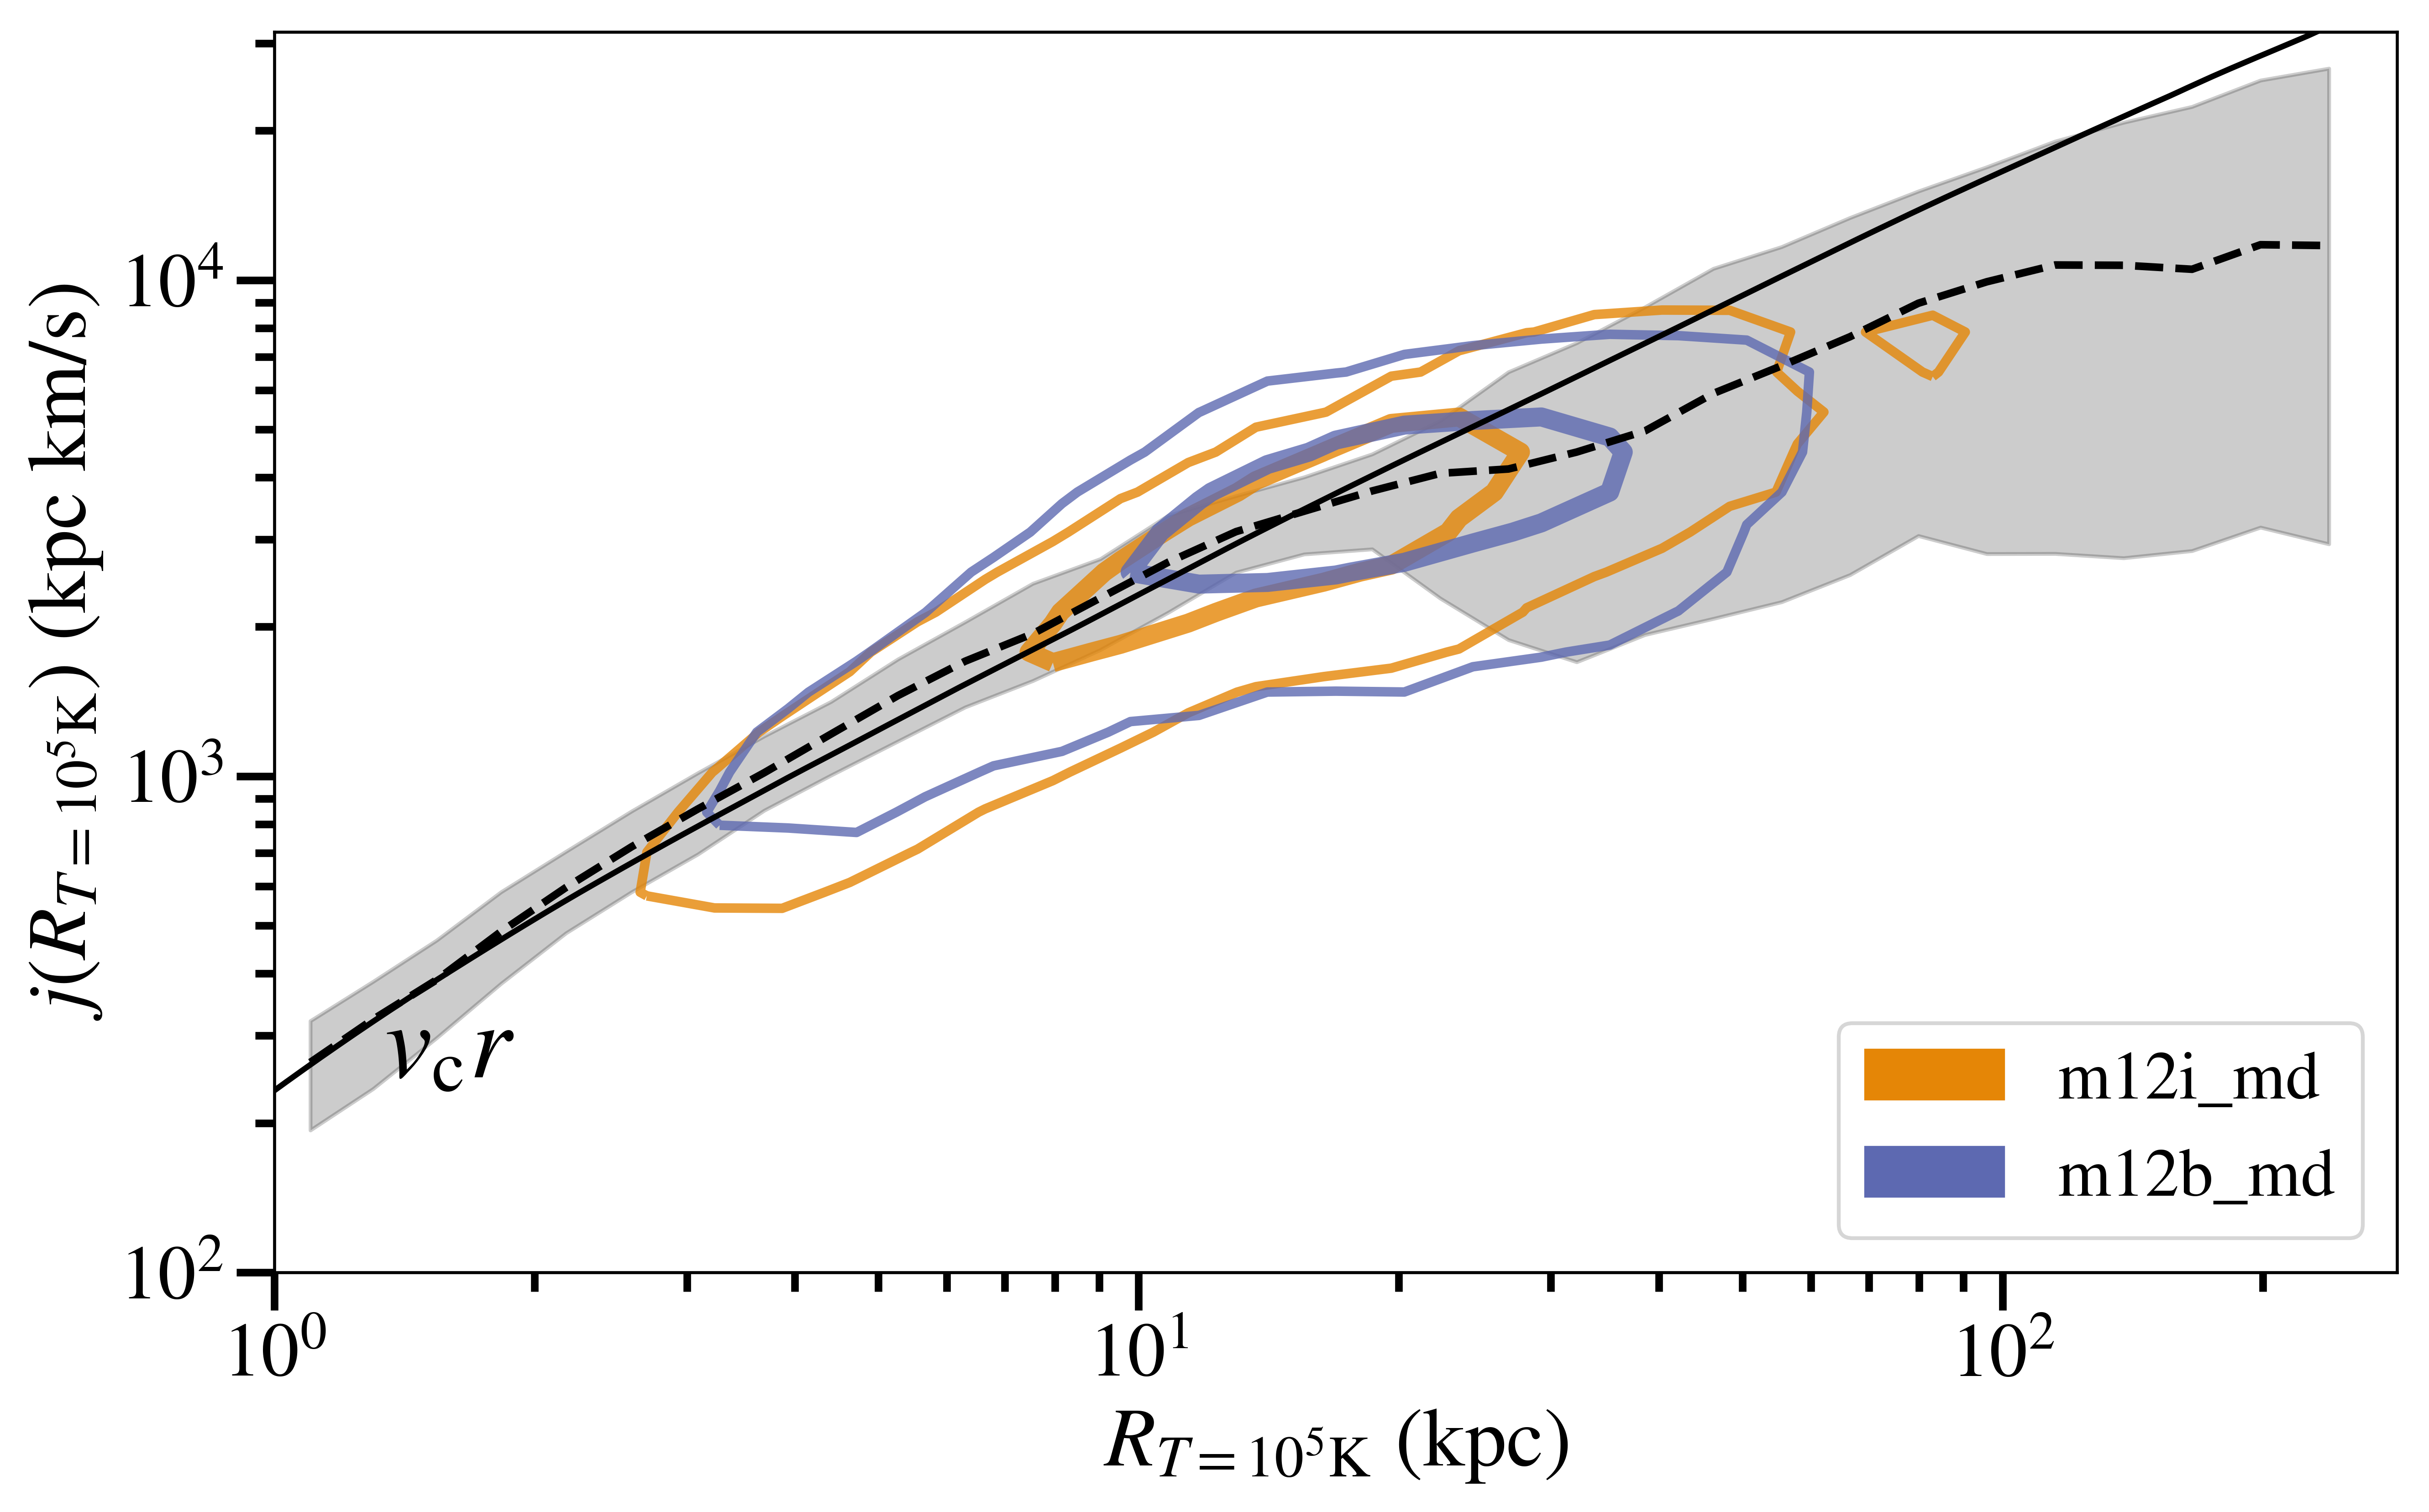
\includegraphics[width=\columnwidth]{figures/j_vs_rcondense.png}
%     \caption{
%     Distribution of $\Rcon$ vs j($\Rcon$) for four FIRE-2 halos with $L(z=0) \sim L^\star$.
% Thick (thin) contours enclose values for 50\% (90\%) of the accreted gas particles.
% The angular momentum as a function of radius for all gas in \texttt{m12i} at $z=0$ is displayed as a dashed line (the median) and shaded regions (5th-95th percentiles).
% \textbf{
% Maybe delete this figure later, because it's only relevant for simulations that have a wide distribution of $\Rcon$, which are only the artificially wide non-md runs.
% }
% \textbf{Is the 100 kpc-cooling gas related to satellite galaxies?}
% \textbf{Try changing shaded region to only hot gas instead of all gas.}
% \textbf{Try histogram of r/(j/vc) instead, to demonstrate that that decreases the spread.}
% \textit{
% In all halos the distributions are consistent with $j_{\rm c} = v_{\rm c} r$, i.e. gas cools once circularized.
% This demonstrates that the variable angular momentum of incoming gas drives the width in the $\Rcon$ distribution.
% }
%     }
%     \label{f: jcool vs Rcon}
% \end{figure}

%%%%%%%%%%%%%%%%%%%%%%%%%%%%%%%%%%%%%%%%%%%%%%%%%%


% Don't change these lines
\bsp	% typesetting comment
\label{lastpage}
\end{document}

% End of mnras_template.tex
